\chapter{Design and Implementation}
\begin{quote} 
\it This chapter covers the implementation details of the concept, the algorithms. All the simulations are first carried out in MATLAB{\textregistered}/Simulink{\textregistered},including testing and verification. The section also introduces the proposed hybrid algorithm.
\end{quote}
%\right 

\section{Cell Characterisation}\label{sec:cel_char}
In this section, model building for \ac{DSCs} is discussed. Several models that have been analysed in literature,  usually variations of the Single Diode model or the Double Diode model (discussed in section \ref{sec:SDM},\ref{sec:DDM} and \ref{sec:eDDM}), form the building blocks for the model construction.
 
\subsection{Test Setup}

 In the pursuance of creating a working solar cell model and to validate the algorithm several measurements would need to be performed. The Test-rig consisted of a blacked-out enclosure to suppress interference from ambient light. The Test-rig or Light-box is fitted with an array of evenly spaced white-\ac{LED}s to provide uniform illumination on the Test subject. The \ac{LED}-array is calibrated and temperature controlled so as to provide white light with a known spectra. A high precision Lux Meter(\textit{GOSSEN Mavolux 5032B}) is used to measure the  intensity of the light, as perceived by the human eye. The \textit{GOSSEN} serves as a reference for Lux measurement throughout the project. The light chamber is also routinely calibrated against a reference cell to factor-in the variations and degradation of the \ac{LED}s. The intensity of light is varied using a high-voltage power supply. A pictorial representation of the above description can be seen is figure ~\ref{fig:test setup} on the next page. \\



 \begin{figure}[H]
	  \begin{center}
		  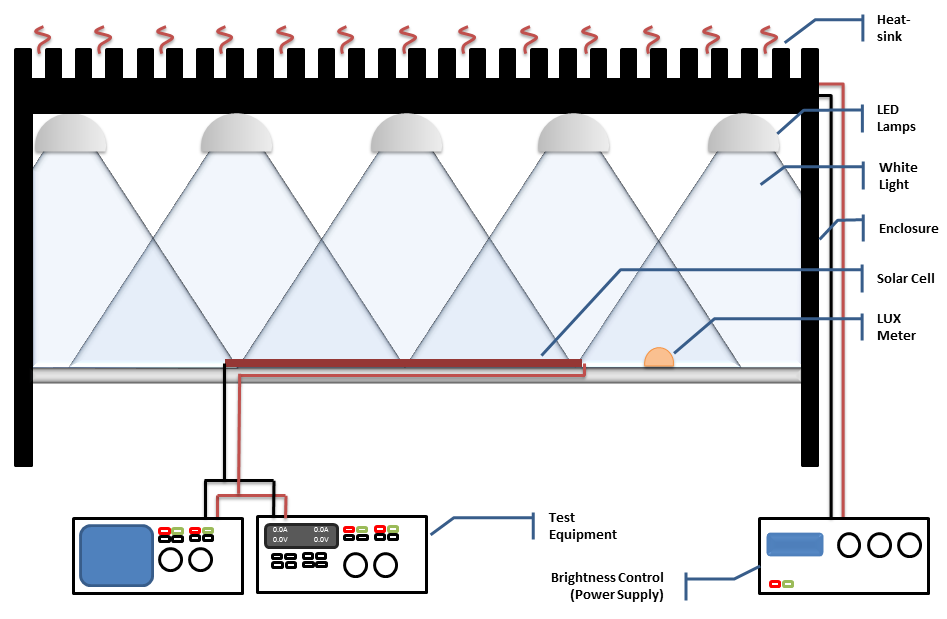
\includegraphics[width=\textwidth]{images/Light_Box}
		  \caption{Test Setup }
		  \label{fig:test setup}
	  \end{center}
  \end{figure}
  

Electrical models for solar cells are frequently found in literature \cite{vignati2012solutions} and \cite{yong2008modeling} among others (discussed in section \ref{sec:SDM} to \ref{sec:eDDM}). However \ac{DSCs} come in many different flavours - dissimilar electrolytes \& electrodes; additional layers and junctions. Added to this, the fact that due to the near impossibility of accurately measuring the multitude of variables of a proprietary commercial cell for this research work, a model was constructed by placing a the test cell under a battery of varied illuminations (0 - 5050 Lux) shown in figure ~\ref{fig:Voltagevlux} (illumination on the X-axis and voltage on the Y). This resulted in a surface that closely resembles the cell's operation under real world conditions. Particular attention was paid to low light conditions which is to be expected for indoor illuminations ( < 2000 Lux). As \ac{DSCs} display very stable output across temperature ranges found indoor \cite{lee2010high}, the above model was made independent of temperature variations.

 \begin{figure}[H]
  \begin{center}
	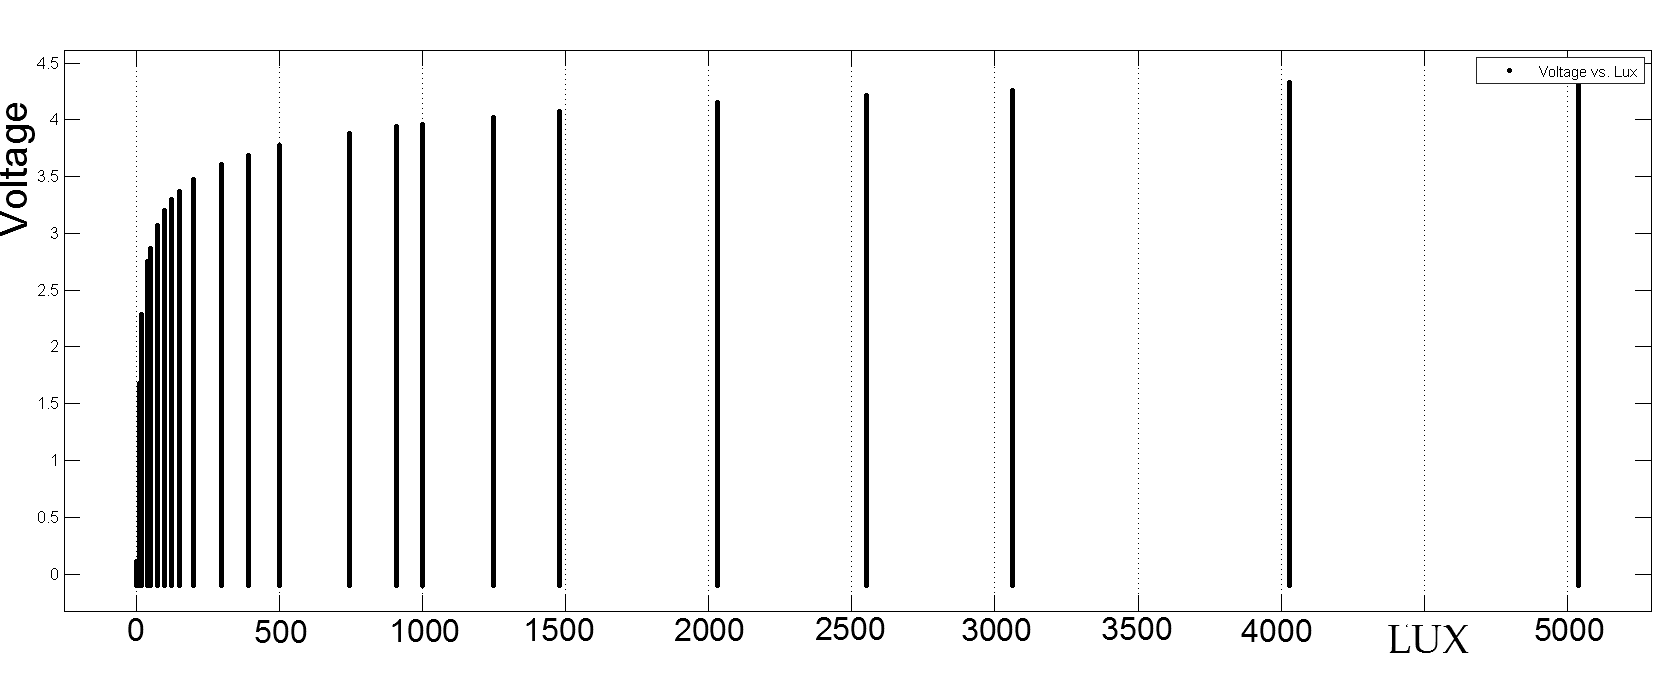
\includegraphics[width=0.9\linewidth]{images/Voltagevlux}
	\caption{Spread of measured Illumination vs Voltage  }
	\label{fig:Voltagevlux}
  \end{center}
 \end{figure}
 The cell-under-test is connected to a \ac{SMU}. \ac{SMU}s have flexibility in their outputs, to be classified as having four-quadrant outputs, they must be able to source power as well as sink power. Sourcing power refers to providing the stimulus for a circuit, and sinking power refers to dissipating power that is being applied by an external active component such as a battery, a charged capacitor, or another power source \cite{NI_SMU} - a solar cell in our case.
 \begin{figure}[H]
	  \begin{center}
		  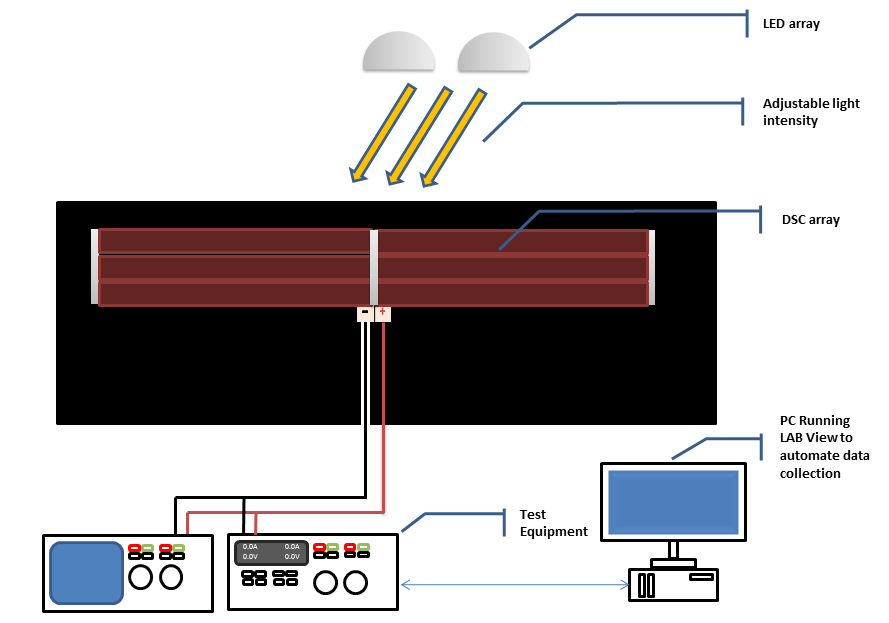
\includegraphics[width=\textwidth]{images/Cell_under_test}
		  \caption{Cell Characterisation }
		  \label{fig:Cell_U_test}
	  \end{center}
 \end{figure}
 As the sink-potential is increased in tiny increments (0.005 V), starting from  0 V to V\textsubscript{OC} and beyond, the cell is forced to operate at the Sink Voltage resulting in the I-V graph depicted in figure ~\ref{fig:2500luxIV}. When the above is repeated for several different light intensities we get a three-dimensional surface shown in figure ~\ref{fig:luxIV100_2500} on page~\pageref{fig:luxIV100_2500}. Note that, V\textsubscript{OC} is the maximum voltage available from a cell. This occurs when the cell produces zero current (when the graph intersects the \textit{x}-axis).\\
 
  \begin{figure}[H]
	  \begin{center}
		  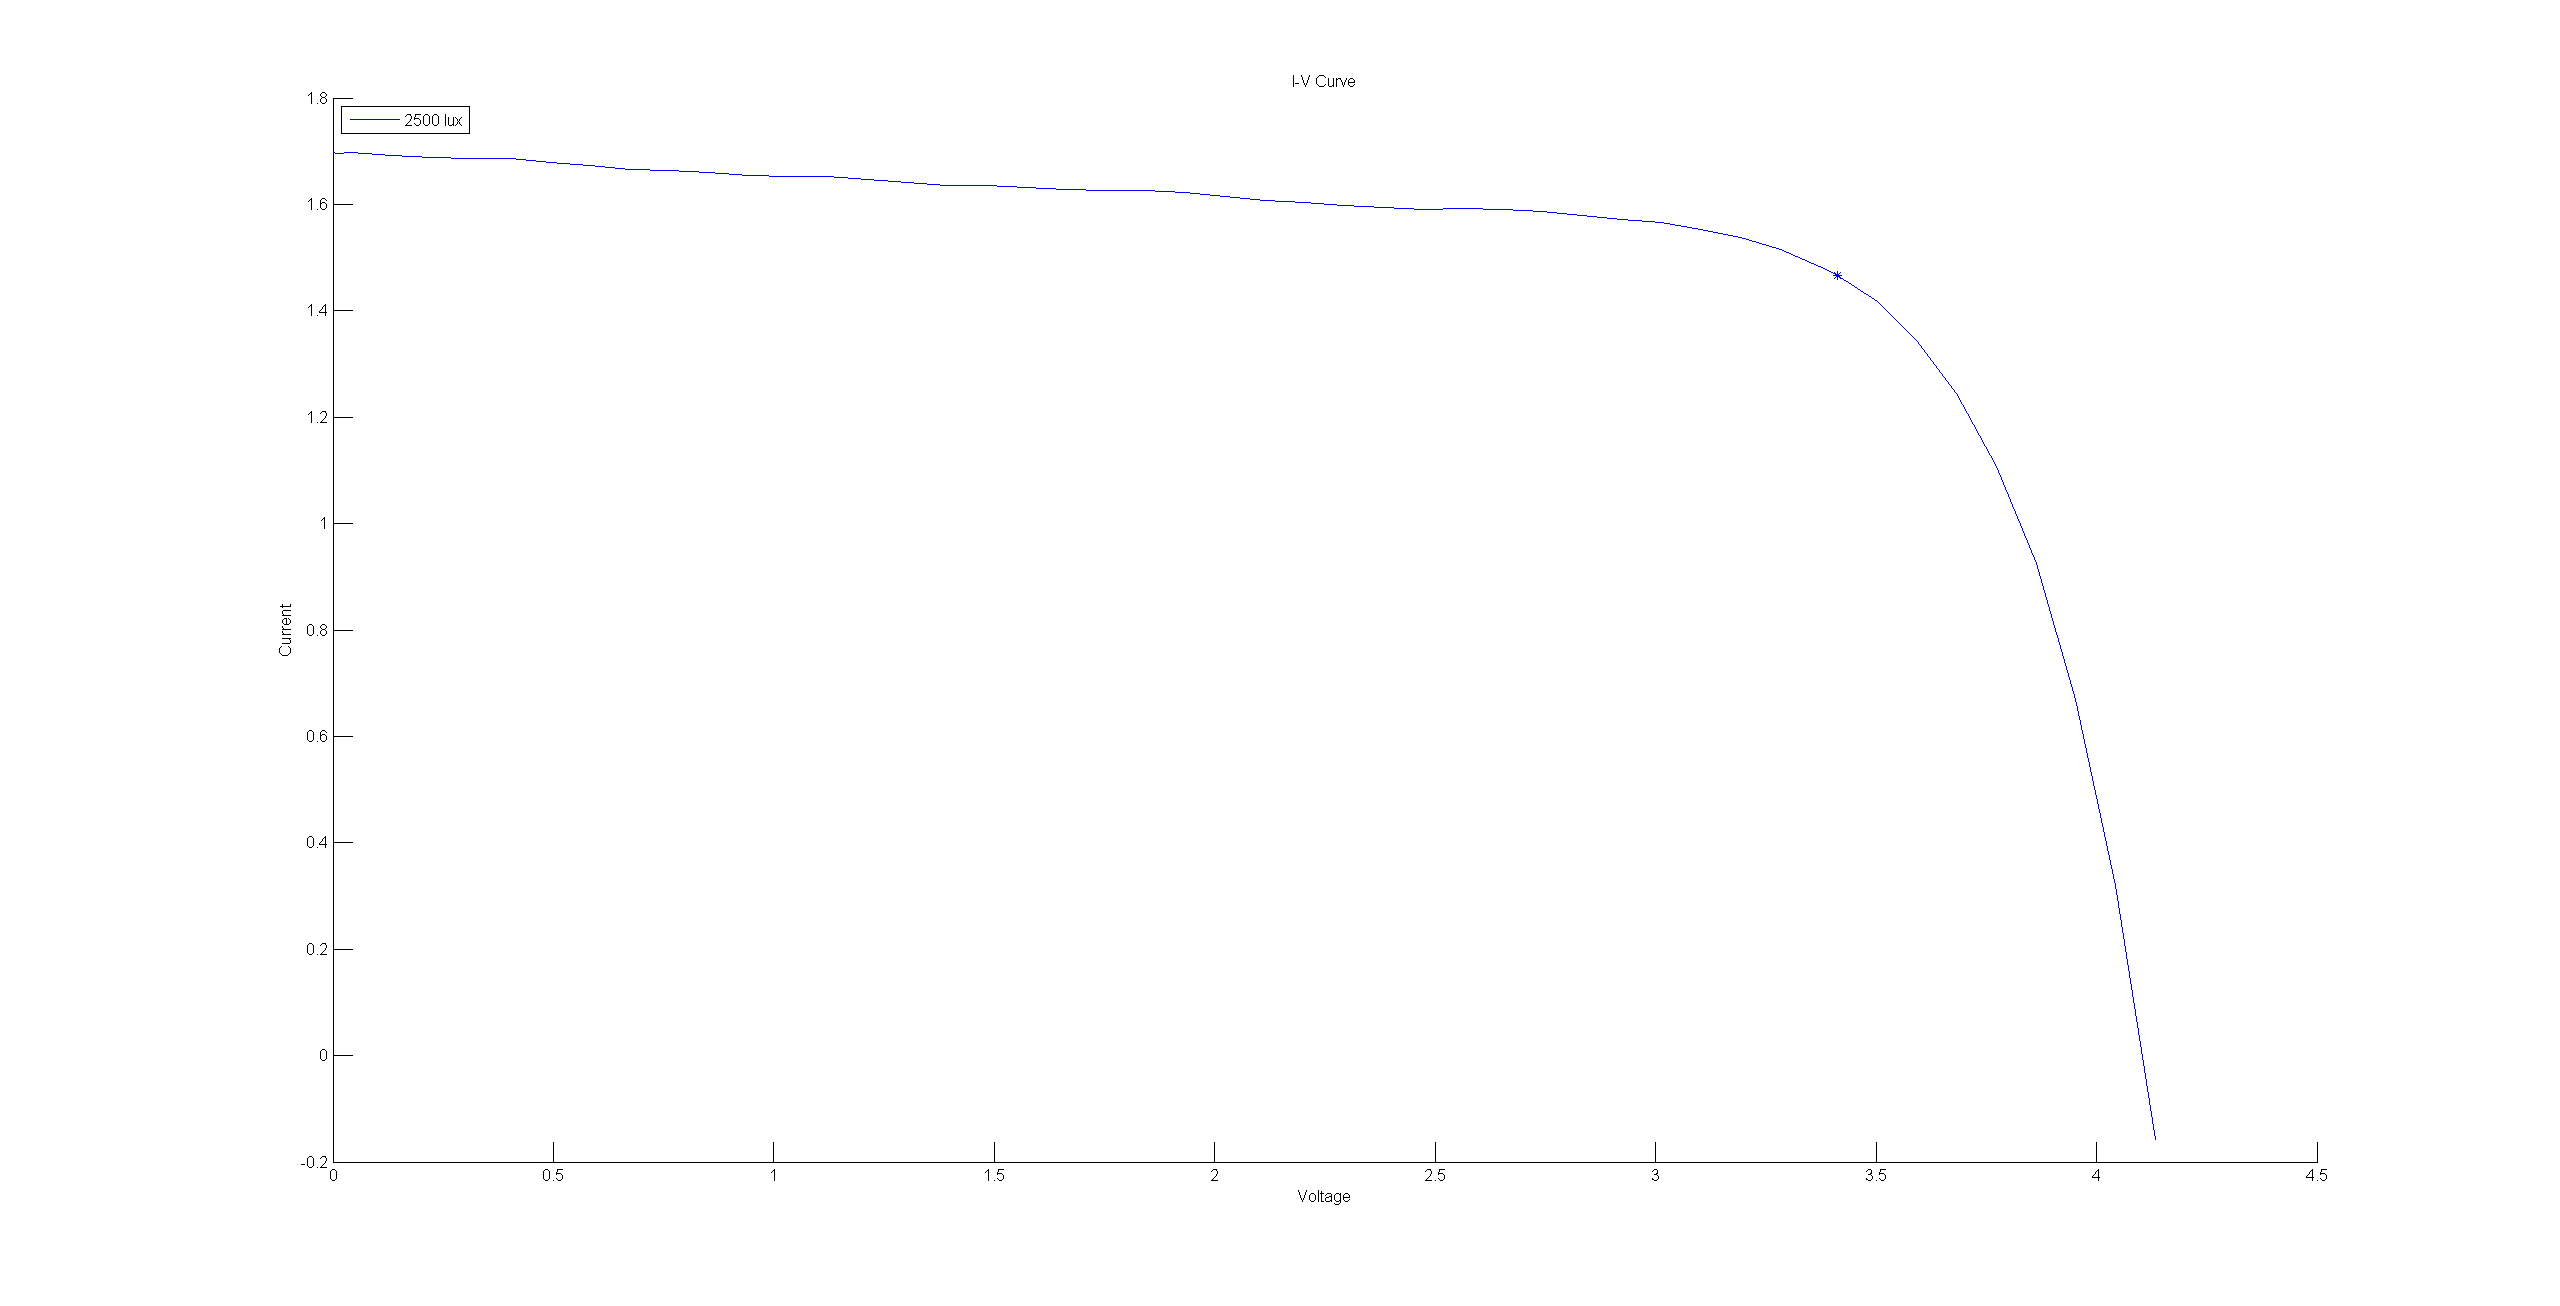
\includegraphics[width=1.1\textwidth]{images/single2500_IV}
		  \caption{I-V curve for the array at steady illumination}
		  \label{fig:2500luxIV}
	  \end{center}
  \end{figure}
  
\begin{figure}[H]
	  \begin{center}
		  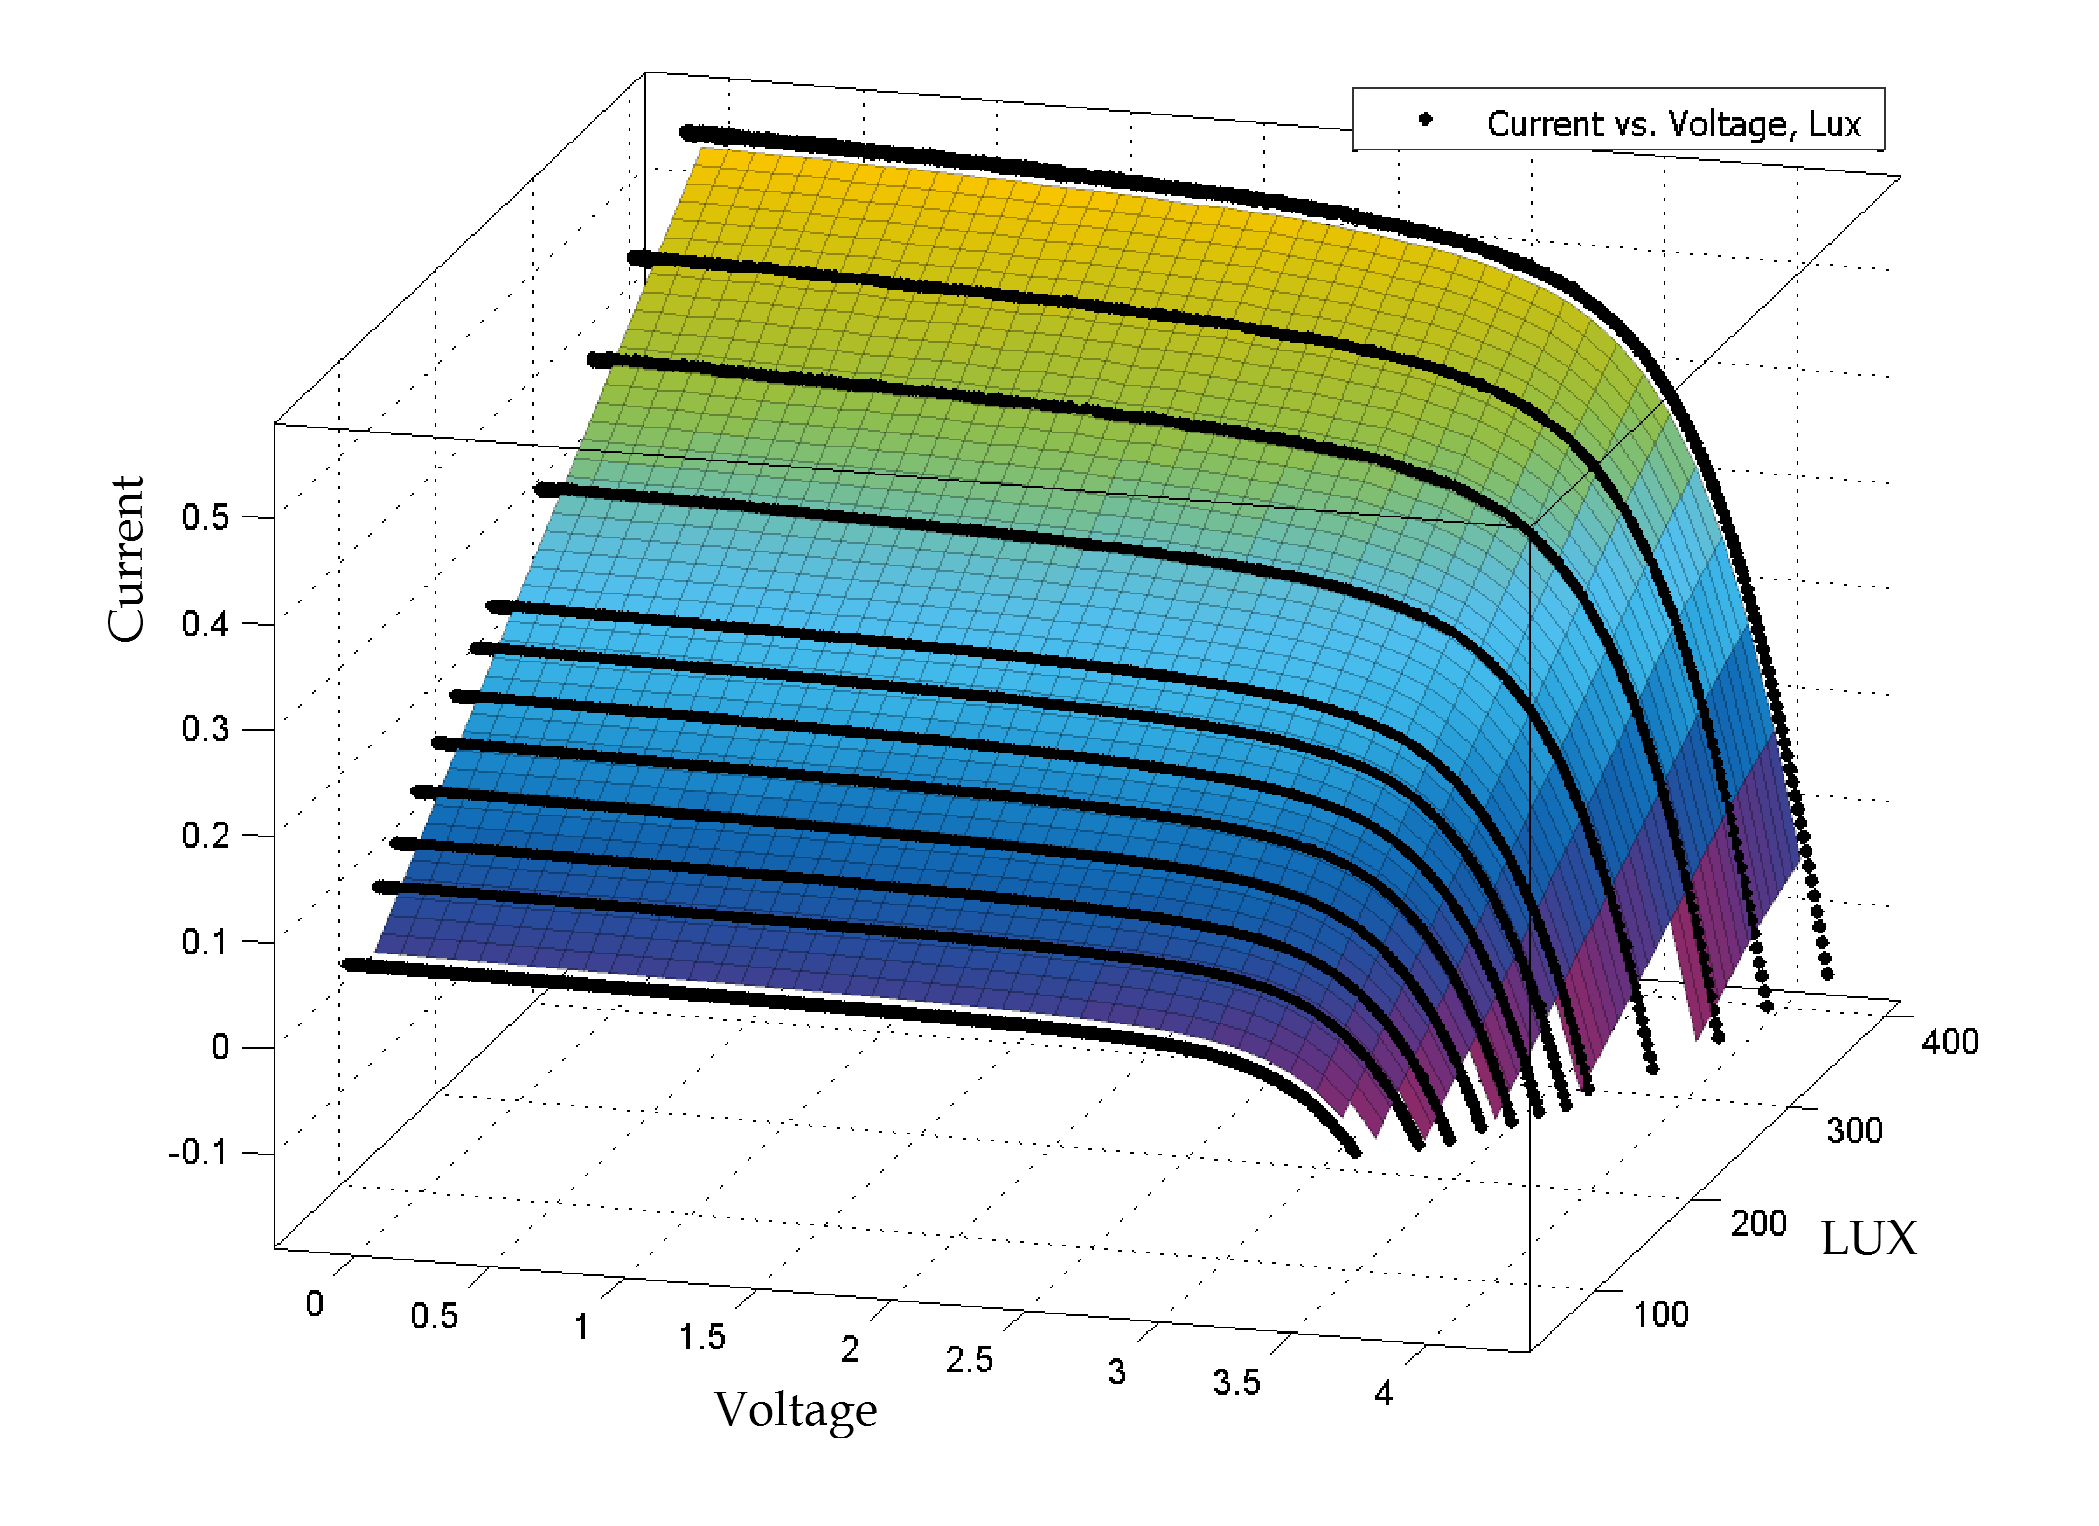
\includegraphics[width=0.8\textwidth]{images/I-V-lux}
		  \caption{I-V curve for the array at varying illumination}
		  \label{fig:luxIV100_2500}
	  \end{center}
  \end{figure}

\section{Modelling and Simulations}\label{sec:mod_sim} 

The three-dimensional surface thus created in the section above acts as a function, a \textit{look-up table} of sorts, for a given illumination and voltage; the function computes an appropriate value for the cell's current . To convert continuous voltage values to discreet values, transfer functions are used. The \ac{DSCs} subsystem is represented in figure~\ref{fig:PV_block_Model}. Capacitor is added in order to accurately mimic the response of \ac{DSCs} under test as discussed in section~\ref{sec:eDDM}. The diode acts as a Snubber, eliminating flyback emf across the inductive load. This sub-system is placed under a mask in the abstract view (Red block), shown in figure~\ref{fig:Model_top} on page~\pageref{fig:Model_top}, in order to simplify operation and for ascetic reasons. The validation of the said model is discussed in section \ref{sec:Validation}. Another \textit{look-up table} provides Open-circuit Voltages ($V_{OC}$) for a given Lux, to be used in certain algorithms. \\

The \textit{Scopes and Outputs} subsection (Green block in figure~\ref{fig:Model_top} ) is used to plot data on to graphs and to push data onto Matlab, for further analysis.\\

The \ac{MPPT} \textit{Controller Block} (figure~\ref{fig:Controller_mod} on page~\pageref{fig:Controller_mod} ) is modelled as a variant subsystem. The variant-control determines which variant is active, and is set before the simulation is started. This arrangement of subsystems makes it extremely easy to switch between and compare the various \ac{MPPT} algorithms without making any alterations to the rest of the model .In figure~\ref{fig:Controller_mod}, \ac{PnO} variant is selected/enabled and other variants are disabled.      

\begin{figure}[H]
	  \begin{center}
		  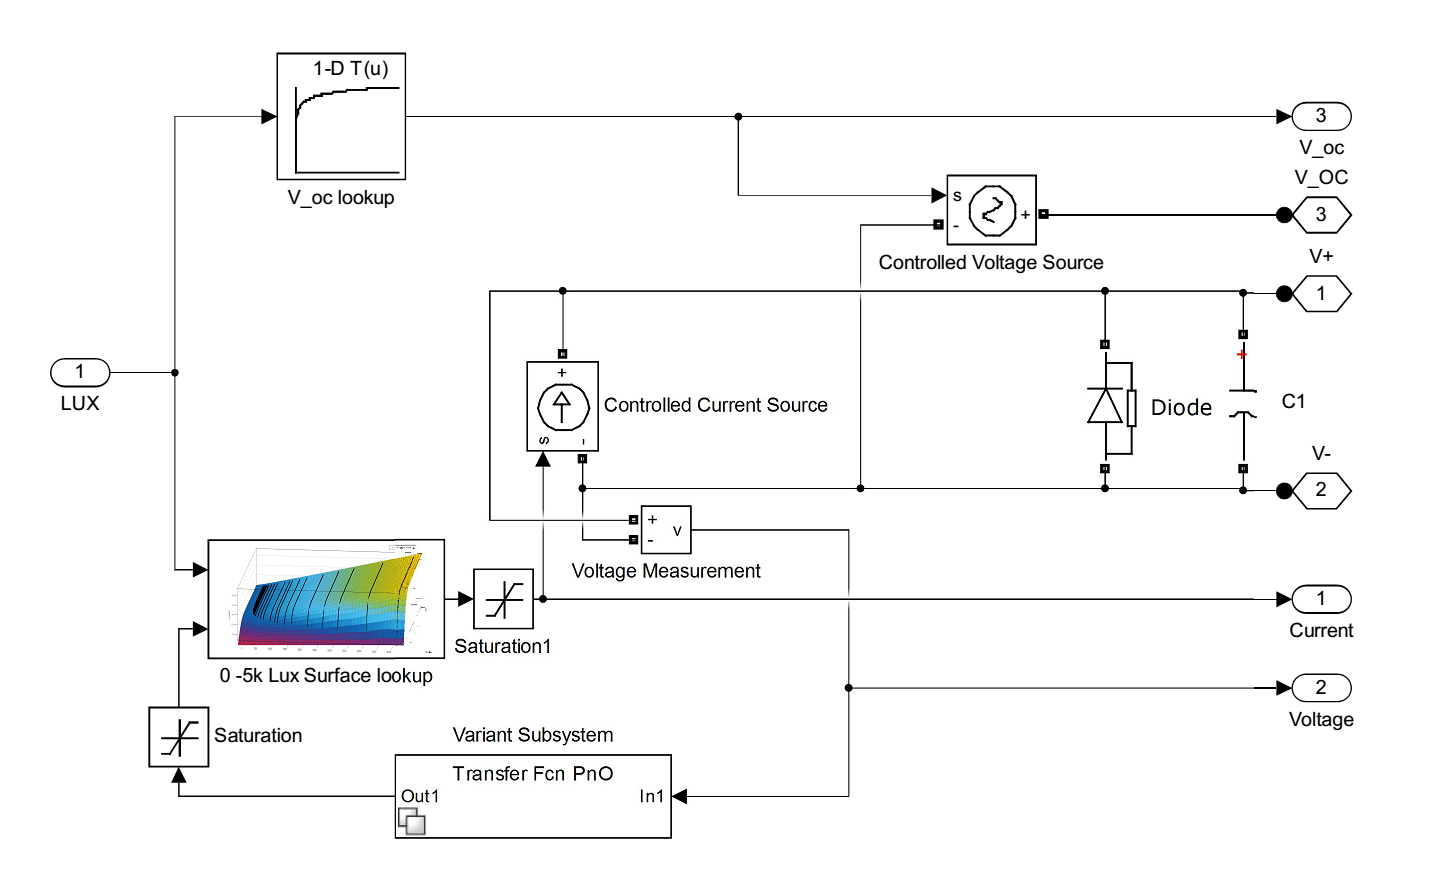
\includegraphics[width=\textwidth]{images/PV_block_Model}
		  \caption{Modelling of the DSC Subsystem block }
		  \label{fig:PV_block_Model}
	  \end{center}
  \end{figure}
  
\begin{figure}[H]
  \begin{center}
	  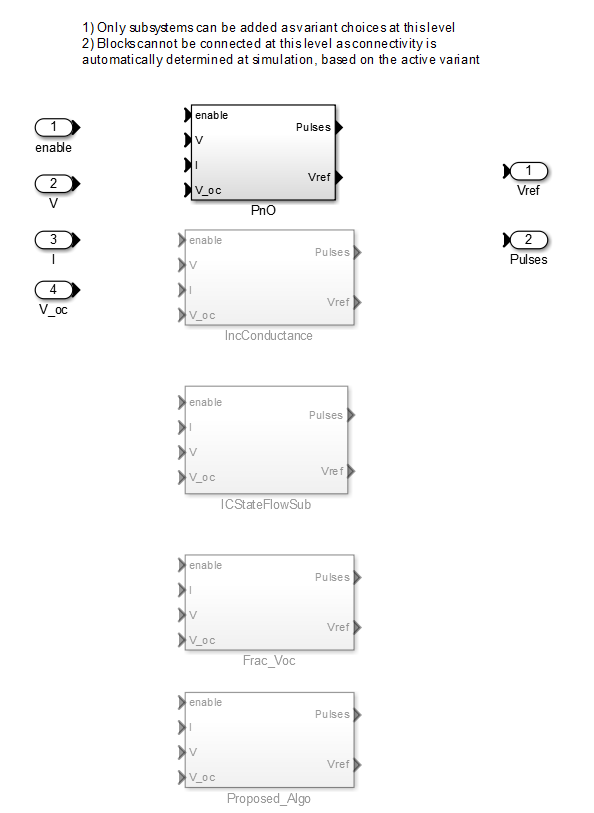
\includegraphics[width=0.55\textwidth]{images/controller_mod}
	  \caption{MPPT controller block}
	  \label{fig:Controller_mod}
  \end{center}
\end{figure}

\begin{figure}[H]
  \begin{center}
	  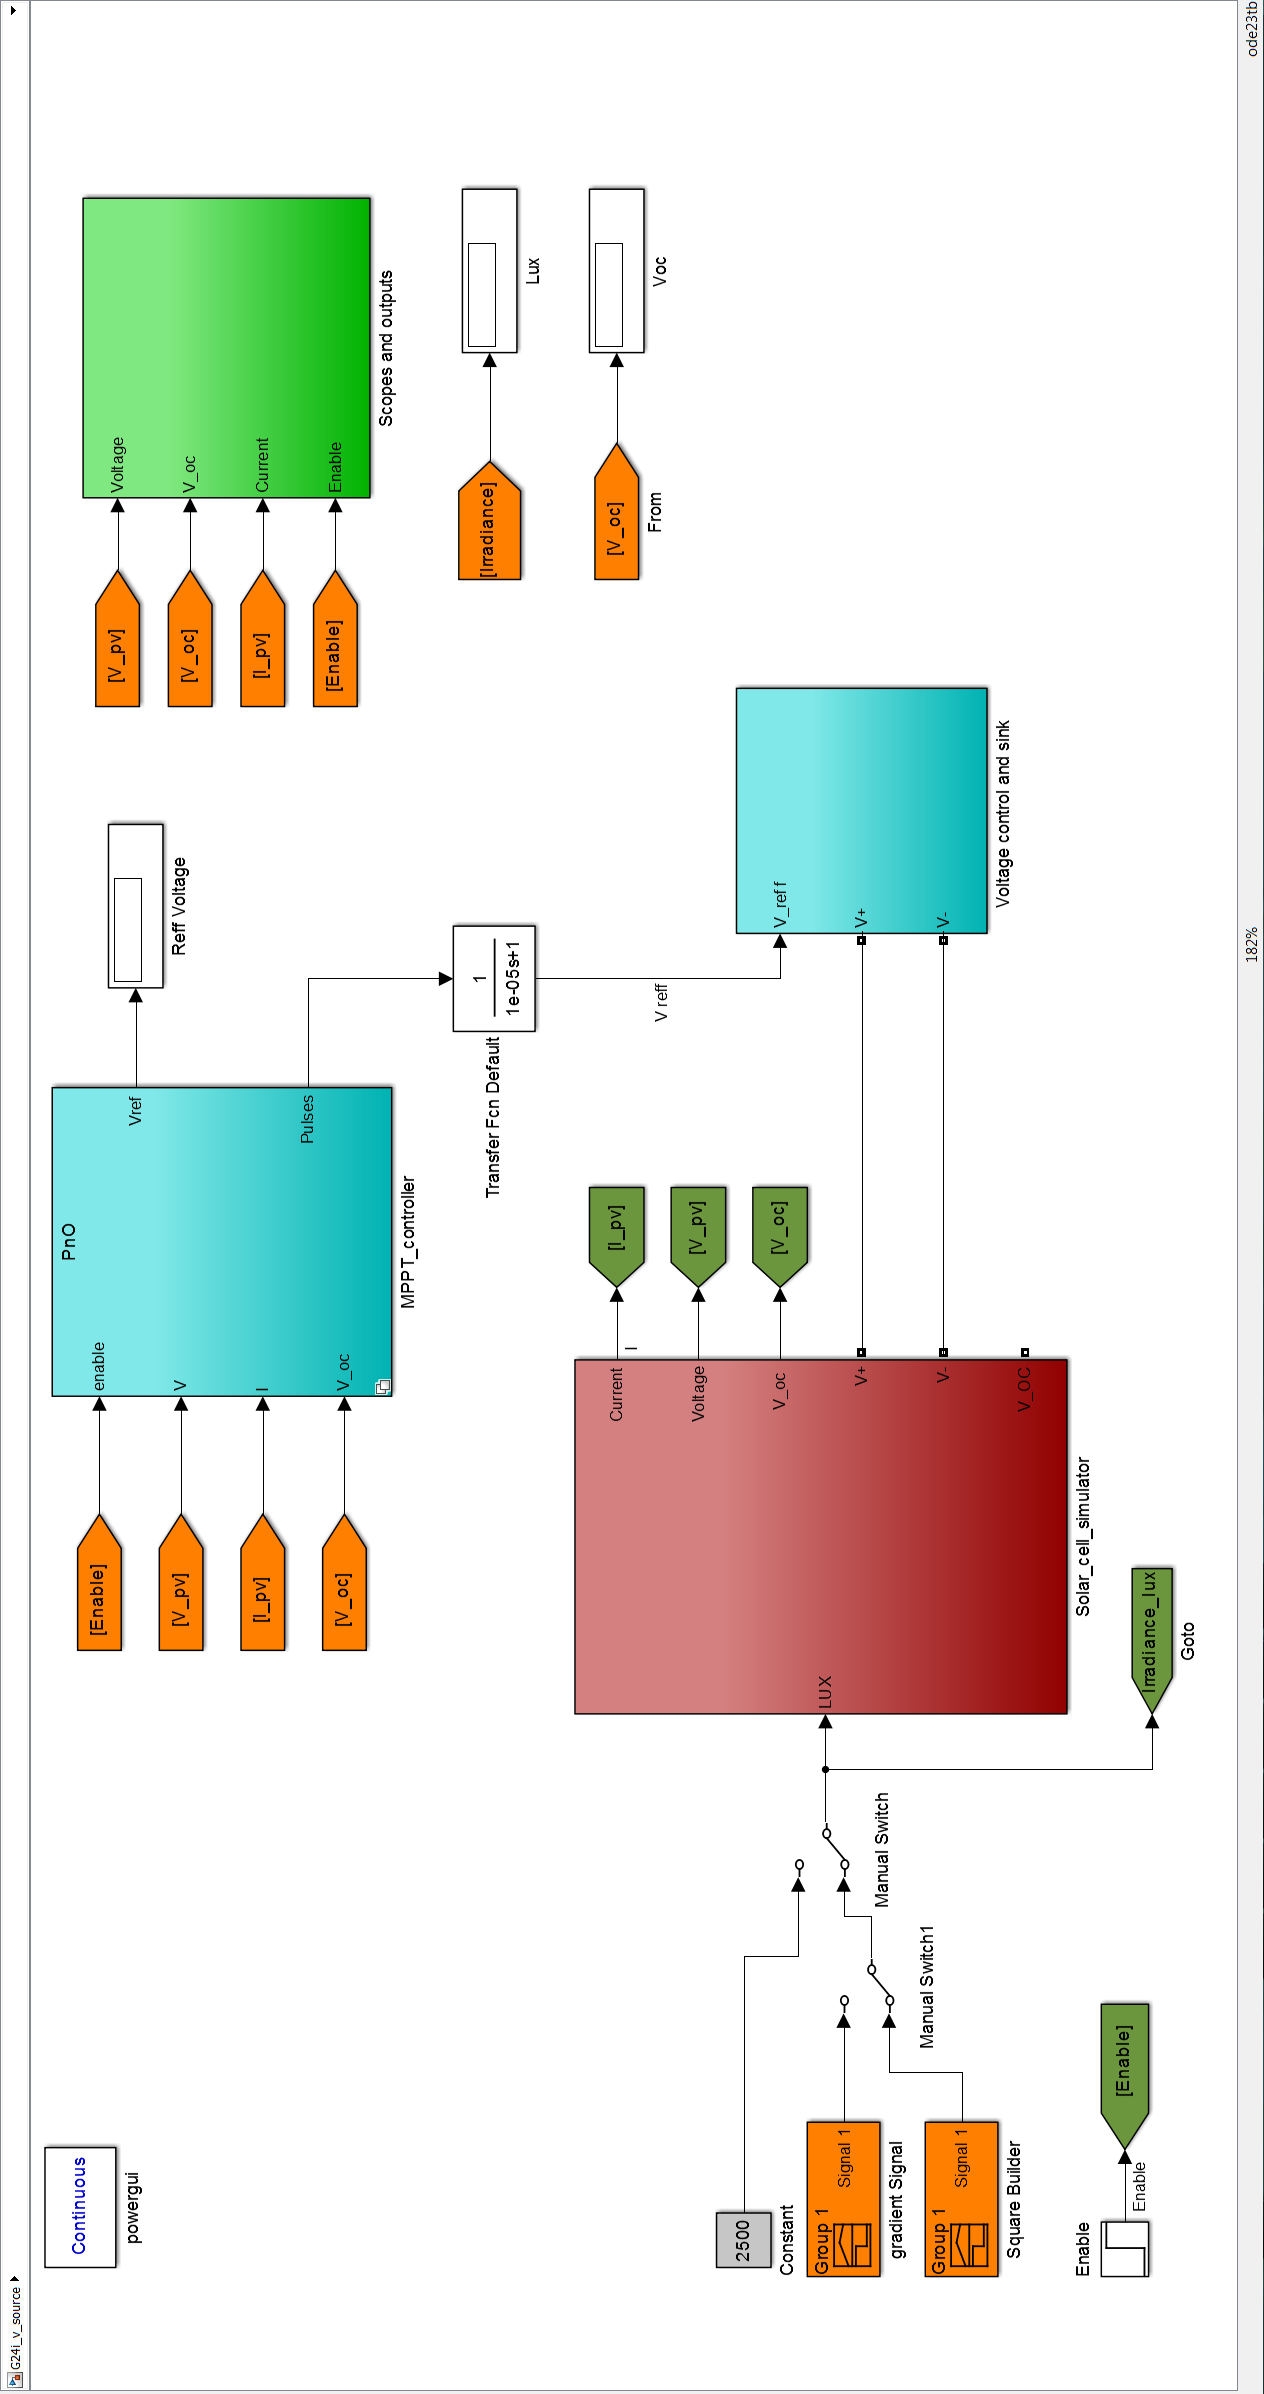
\includegraphics[width=0.8\textwidth]{images/Top_level_mod}
	  \caption{Top level model }
	  \label{fig:Model_top}
  \end{center}
\end{figure}


\section {Validation of the model in Matlab{\textregistered}}\label{sec:Validation} 

Since the credibility of the thesis rests on the accuracy of the model used to compare the different algorithms, therefore, a section is devoted to the validation of the same. The easiest way to do this would be to compare the divergence of Matlab Model (Section:\ref{sec:cel_char}) with the values obtained via experiment.\\

\begin{figure}[H]
	  \begin{center}
		  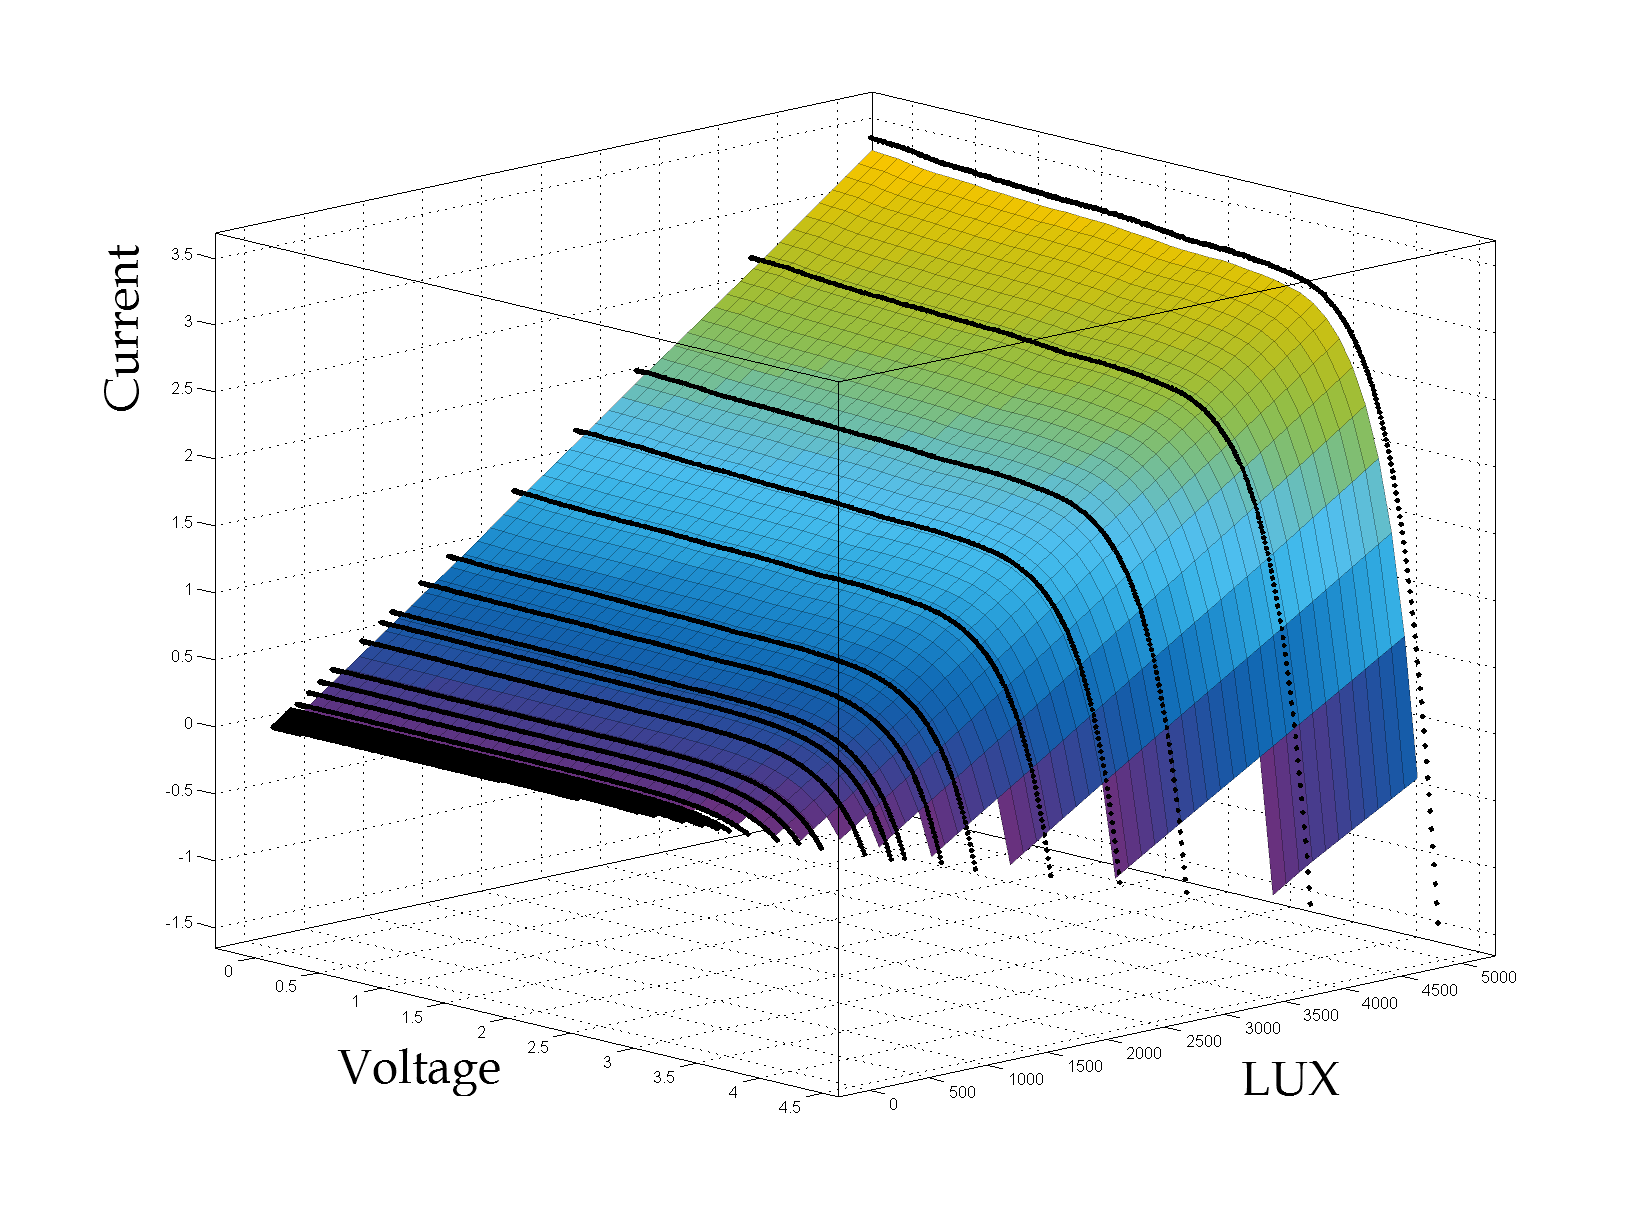
\includegraphics[width=0.85\textwidth]{images/IVLUX_LAB_measured}
		  \caption{3-D representation of the cell's characteristics obtained through measurements in the lab }
		  \label{fig:IVLUX_LAB_measured}
	  \end{center}
  \end{figure}
The model depicted in figure ~\ref{fig:IVLUX_LAB_measured} is generated using experimental data. Measurements were taken with a step size of 0.01V compared to the 0.1V step size for the simulated model(figure~\ref{fig:IVLUX_MOD_gen}), as is evident in the figures. The larger step size makes for faster calculations and smaller \textit{look-up} tables. A fair bit of interpolation is utilised to estimate values for points in between. However, as proved below, these estimations do not introduce any significant errors into the model.\\

On the subtraction of one surface from the other, we are left with figure ~\ref{fig:Diff_Contour}. This resulting 3-Dimensional surface represents the degree by which the two models are different. Figure ~\ref{fig:Contour_map} on page ~\pageref{fig:Contour_map} illustrates this variation in the form of a contour map, in which majority of the discrepancy lies within the error margin of 0.1 mA and the divergence in the area of operation and of interest (0 - 4 V ) is significantly less. This goes to prove the model used in the simulation behaves as close to possible to a real \ac{DSCs} under test conditions.

\begin{figure}[H]
  \begin{center}
	  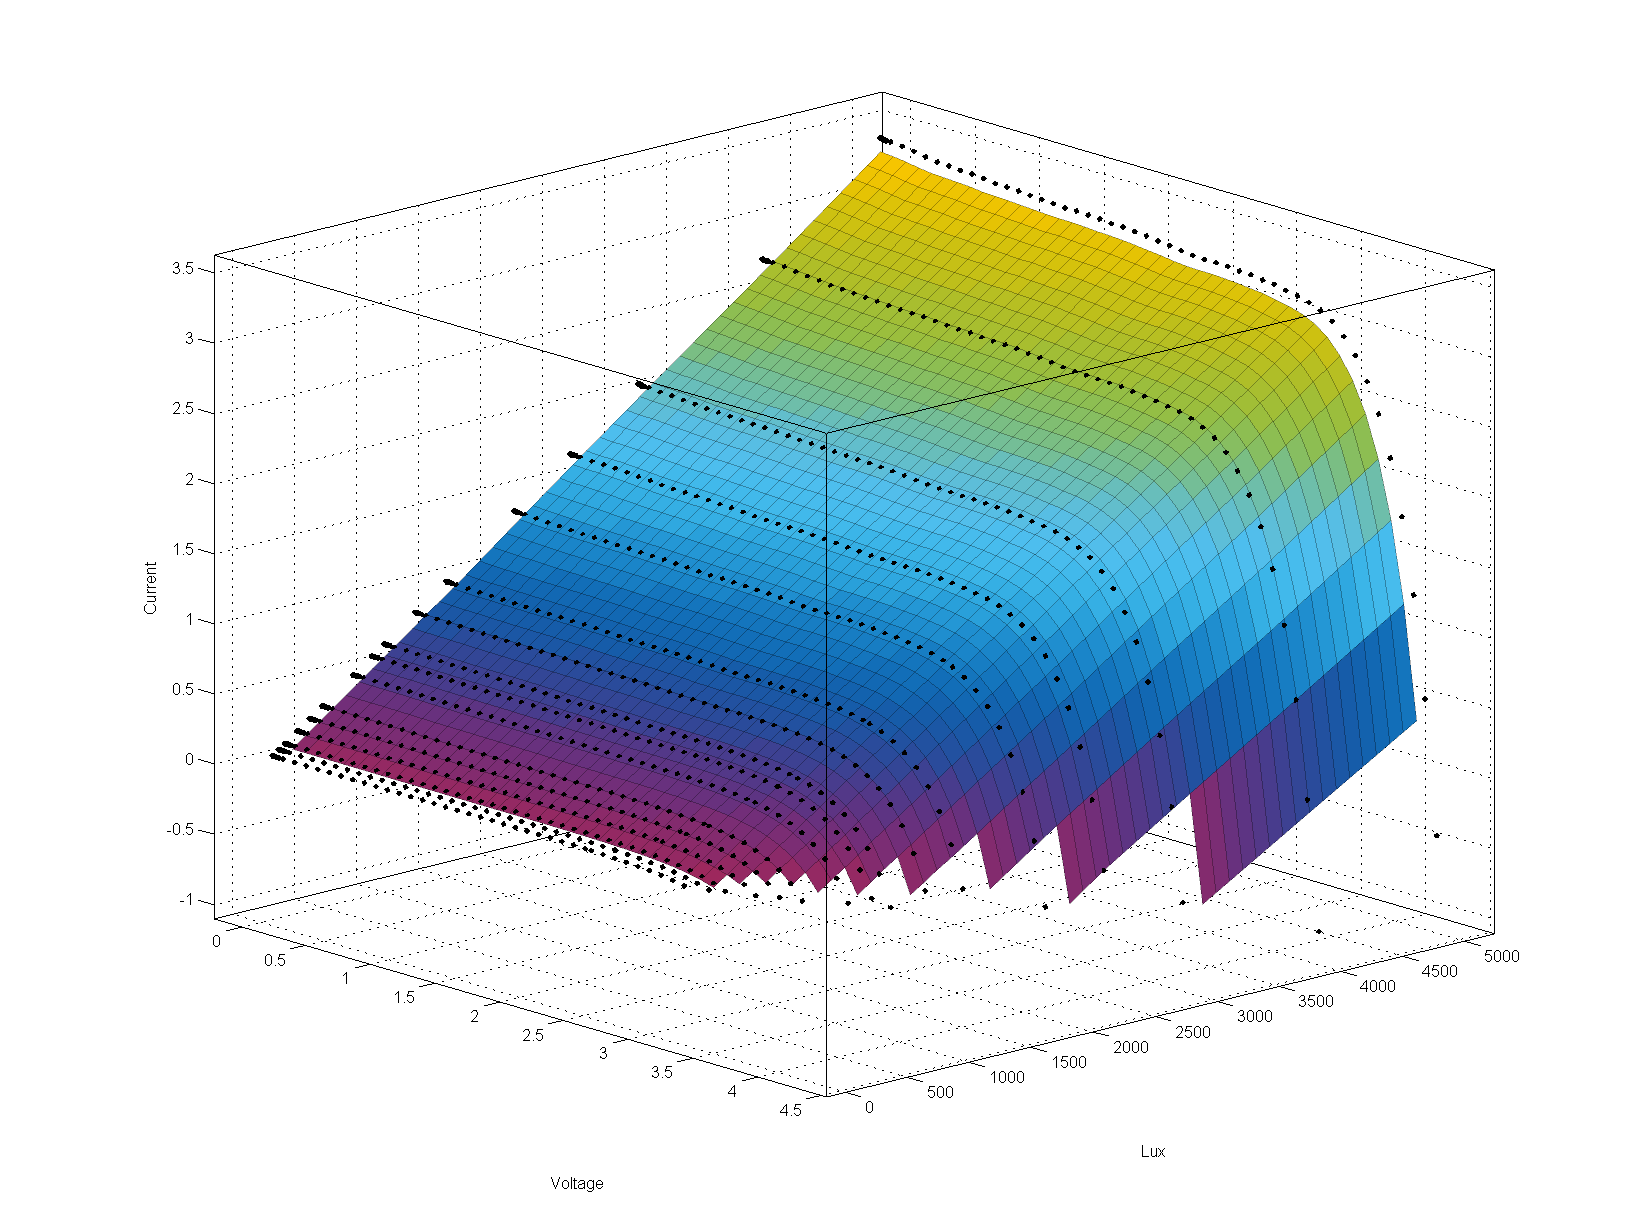
\includegraphics[width=0.85\textwidth]{images/IVLUX_MOD_gen}
	  \caption{Surface generated using the Matlab model developed in section~\ref{sec:mod_sim}}
	  \label{fig:IVLUX_MOD_gen}
  \end{center}
\end{figure}
              

\begin{figure}[H]
  \begin{center}
	  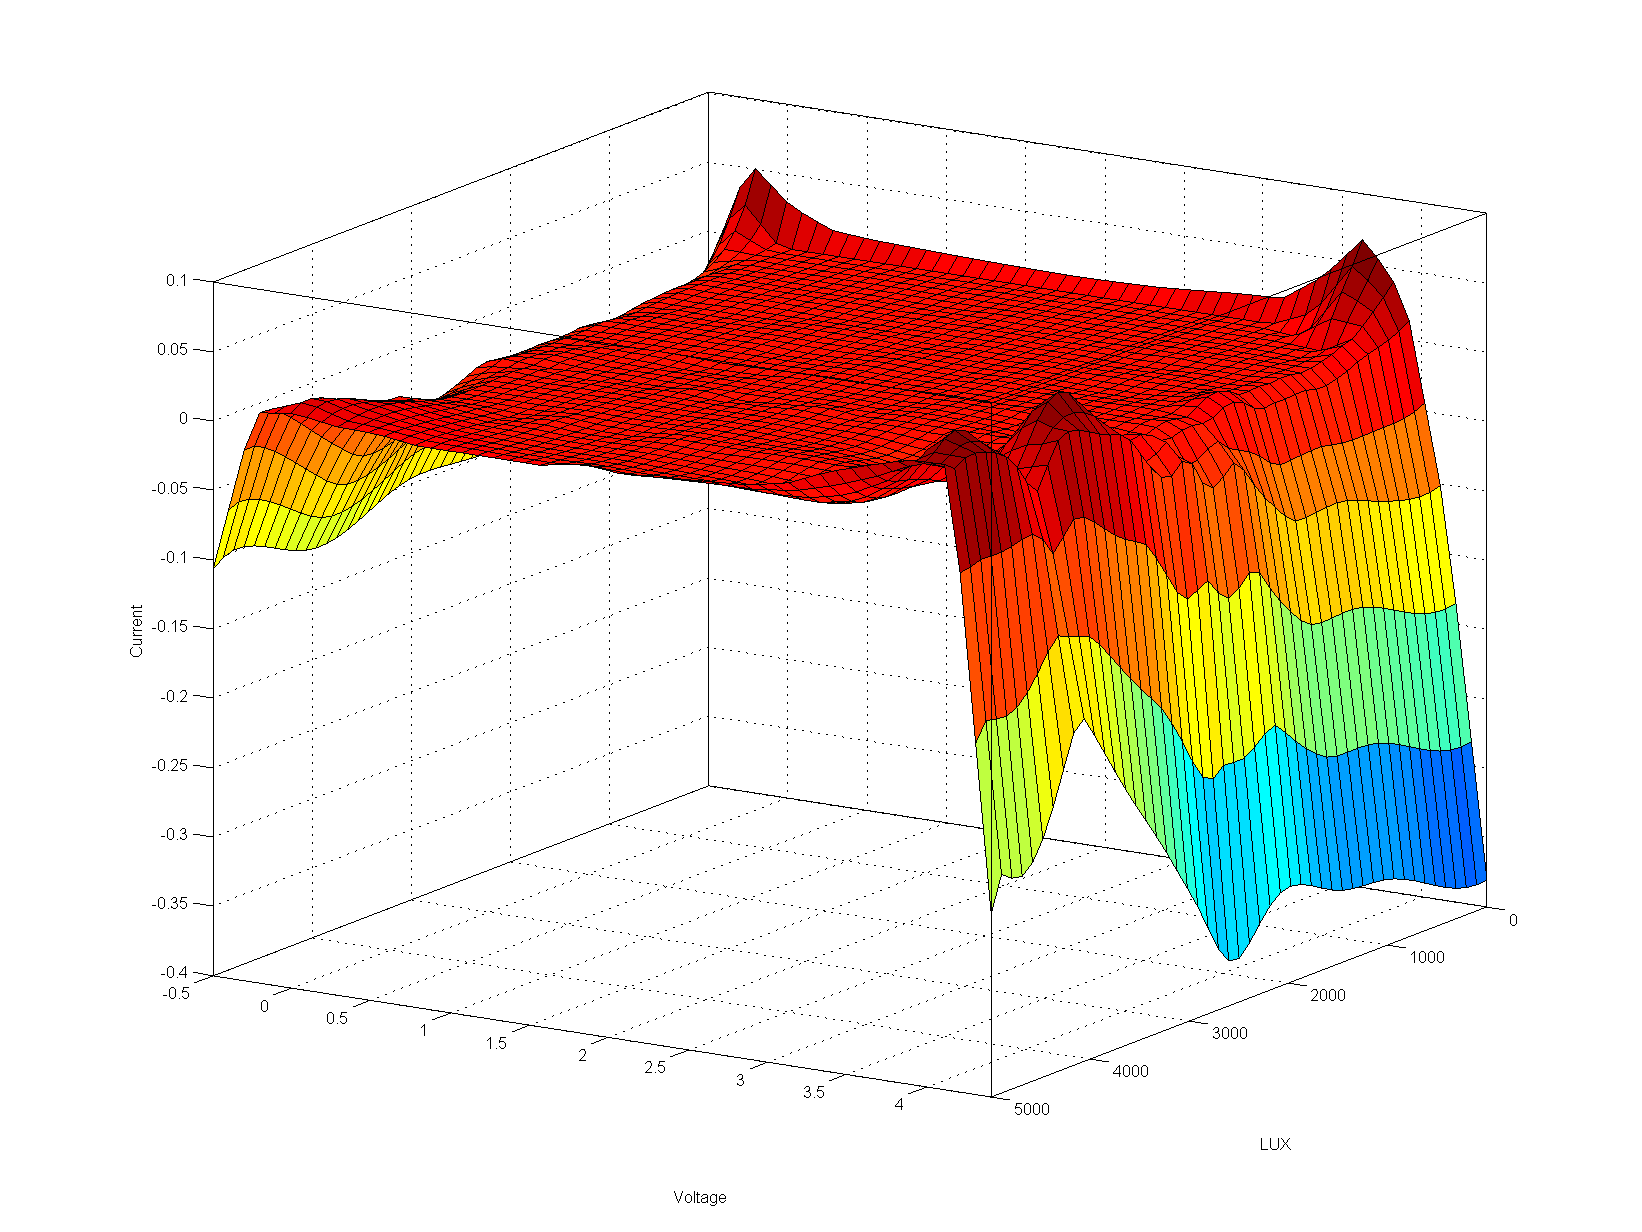
\includegraphics[width=0.85\textwidth]{images/Diff_Contour}
	  \caption{Model resulting from the difference of the two models (Figures ~\ref{fig:IVLUX_LAB_measured} \&~\ref{fig:IVLUX_MOD_gen} )}
	  \label{fig:Diff_Contour}
  \end{center}
\end{figure}


\begin{figure}[H]
  \begin{center}
	  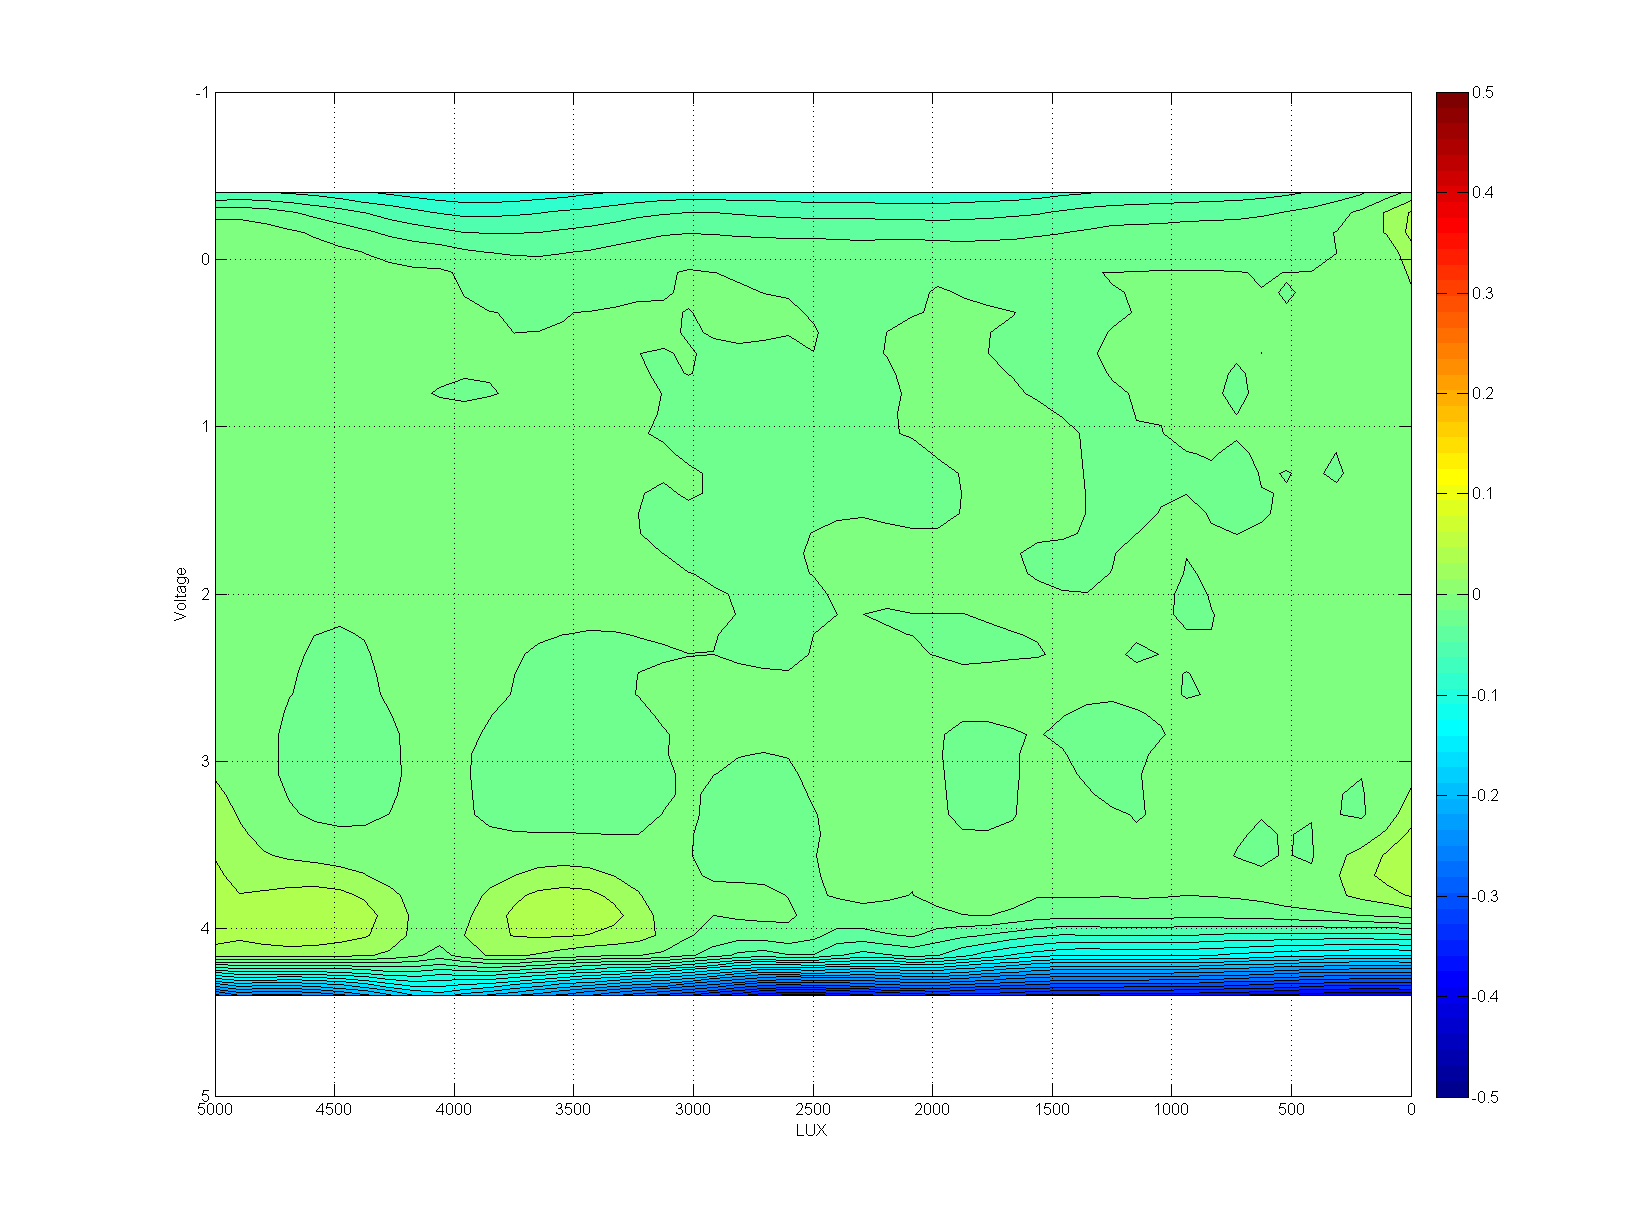
\includegraphics[width=\textwidth]{images/Contour_map}
	  \caption{Contour map of the difference}
	  \label{fig:Contour_map}
  \end{center}
\end{figure}

\section{Proposed Method } \label{sec:proposed_algo_sec}

It has already been established that there exists a relation between $V\textsubscript{MPP}$ and $V\textsubscript{OC}$ and is famously used in the \ac{FOCV} method (section \ref{sec:focv_sec}), given by:

  \begin{equation}
   \begin{aligned}
	  V\textsubscript{MPP}\approx k\textsubscript{i}V\textsubscript{OC}
	  \label{eq:equ_fracoc_proposed}
  \end{aligned}
  \end{equation}  
  
However on second look, the above equation is of the form:
  \begin{equation}
     \begin{aligned}
  	 y = mx
  	  \label{eq:equ_line}
    \end{aligned}
    \end{equation}  
    
which represents an equation of a line passing through the origin but the plot of $V\textsubscript{OC}$ vs $V\textsubscript{MPP}$ shown in figure \ref{fig:Probability_field} on page ~\pageref{fig:Probability_field} obtained via experiments shows that this is not the case. There is in fact an offset that is not taken into account by the \ac{FOCV} Method.\\

Taking this offset into consideration does make \ac{FOCV} method more accurate but this would involve characterising the cell every time before use which would be tedious and not to mention, that this does not take into account cell degradation over time. That being said \ac{FOCV} method does have its advantages - it is relatively simple to implement, it requires only one voltage sensor, measuring voltage is much cheaper and faster than measuring current.\\
\begin{figure}[H]
  \begin{center}
	  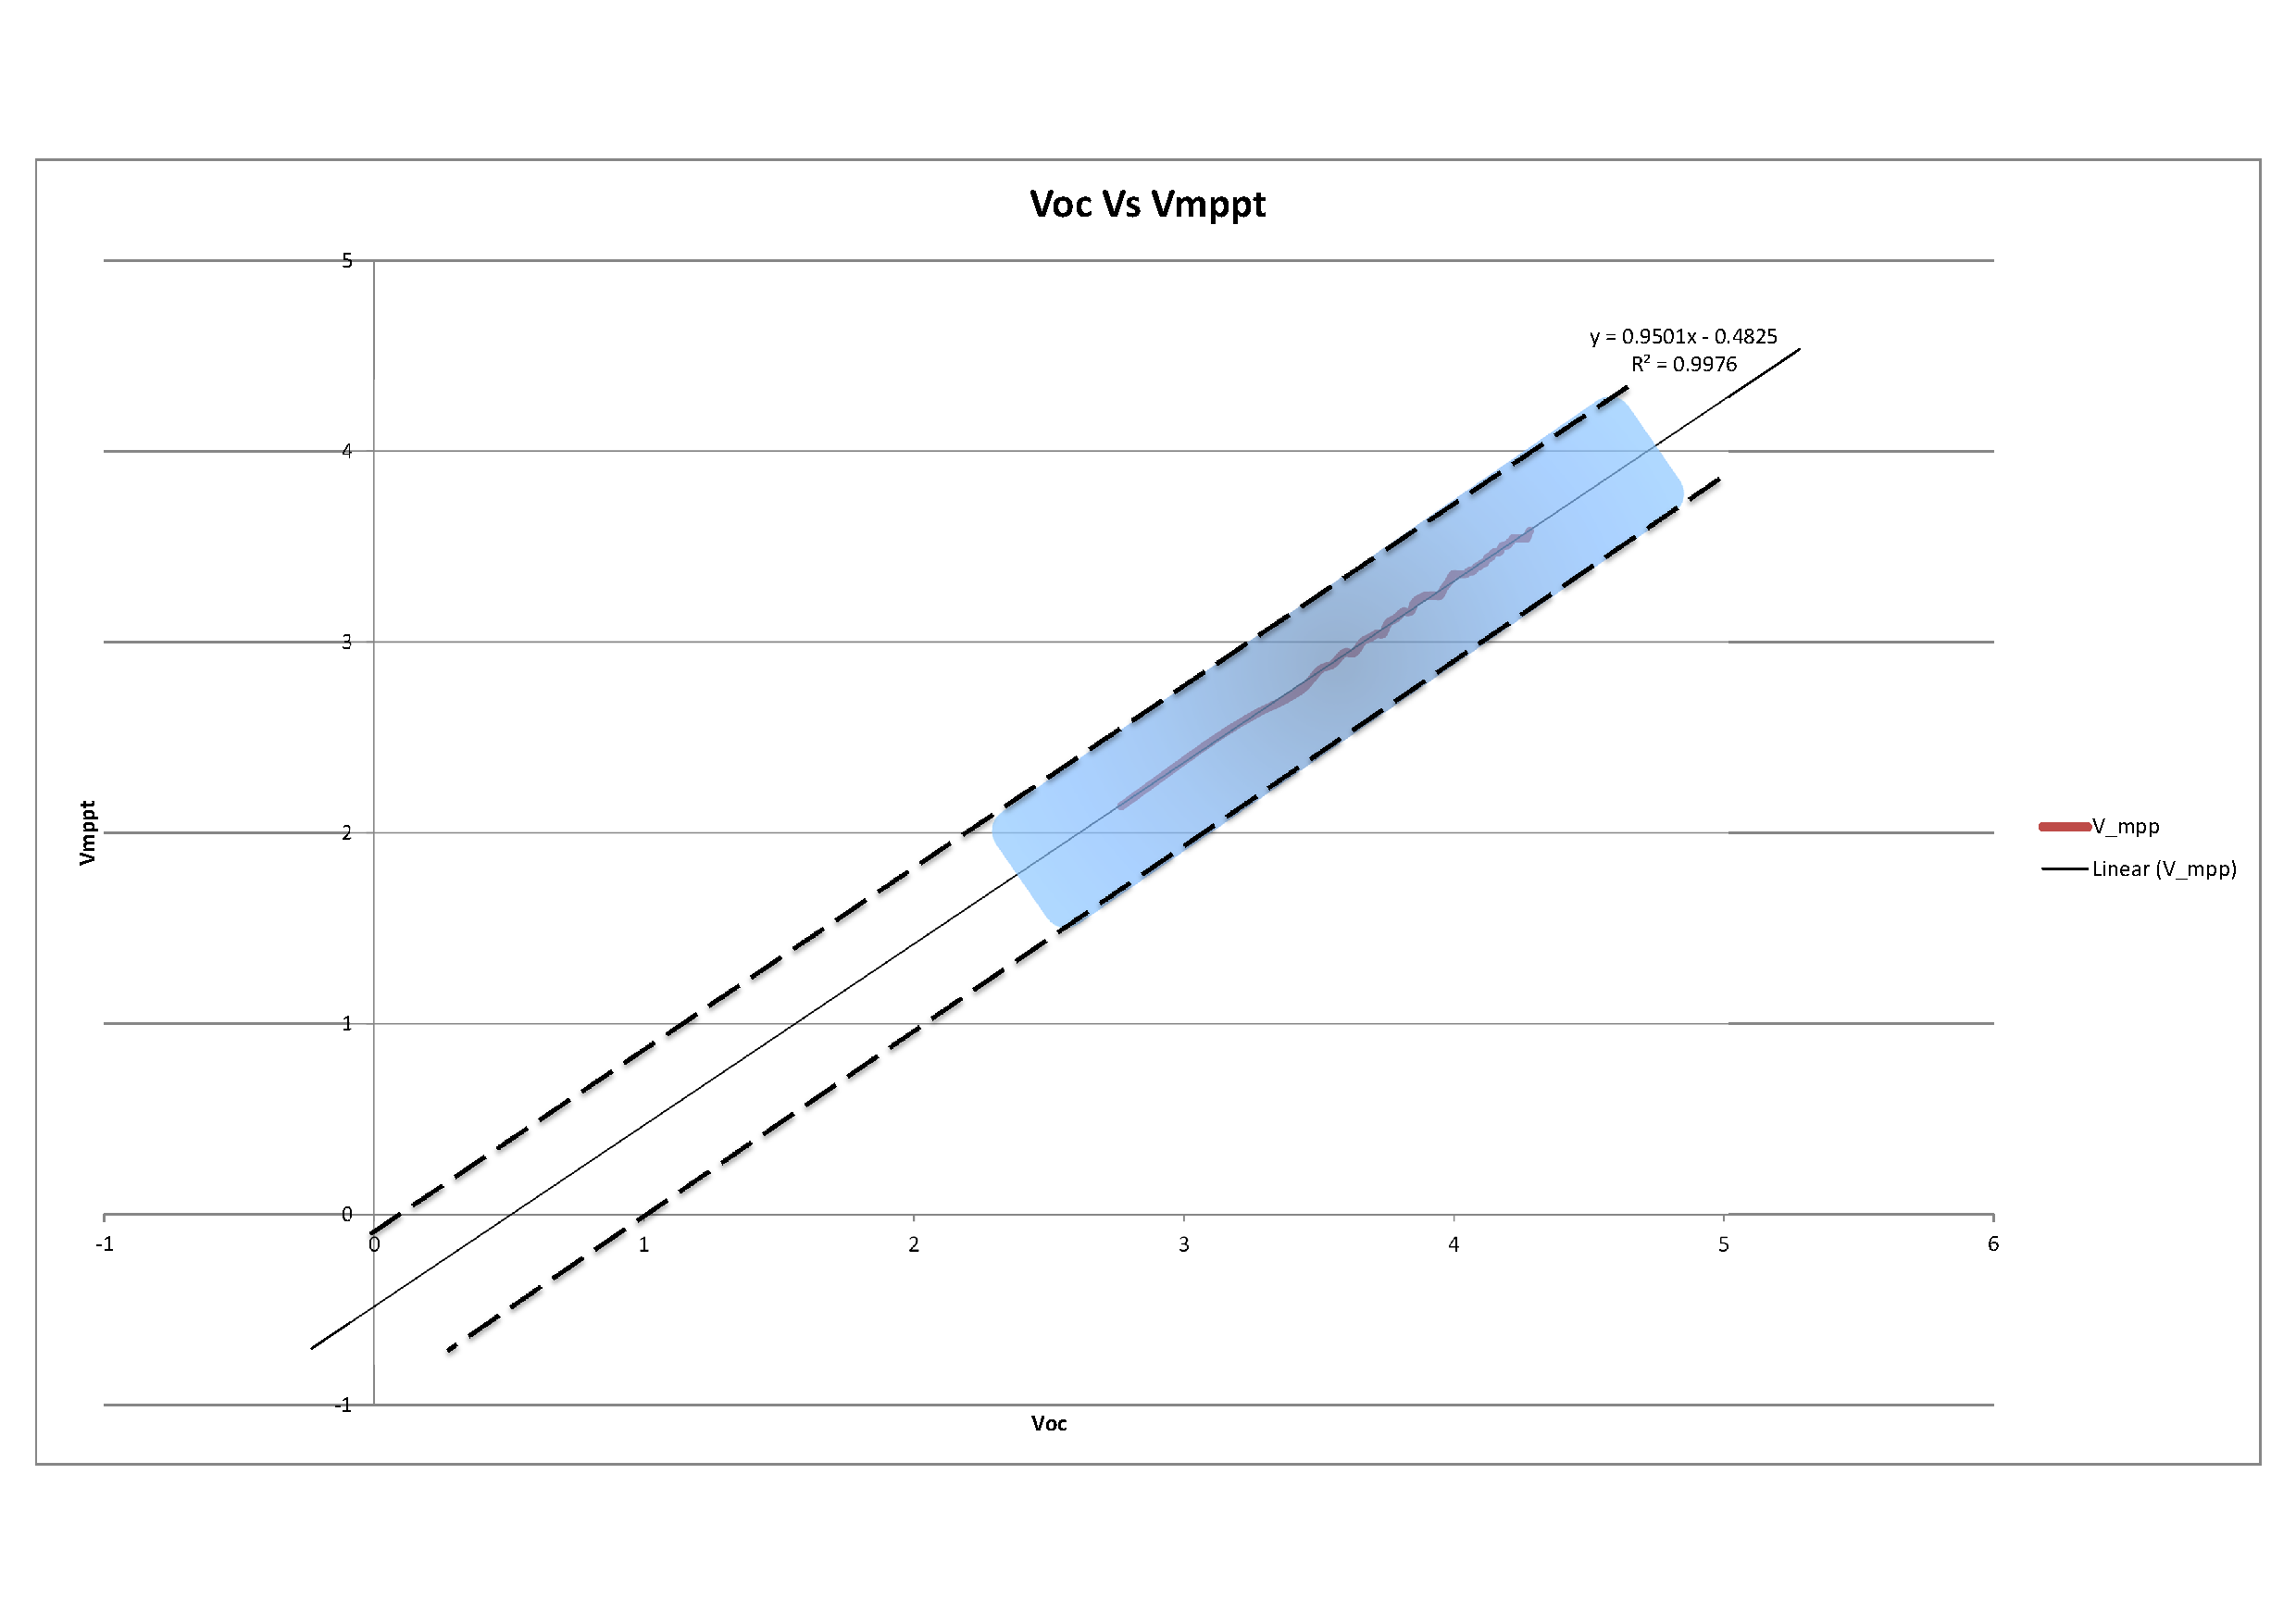
\includegraphics[width=1.1\textwidth]{images/Probability_field}
	  \caption{Probability field }
	  \label{fig:Probability_field}
  \end{center}
\end{figure}

Liu et al.\cite{liu2011fast} found that this relationship (equation~\ref{eq:equ_fracoc_proposed}) does not hold true for all illumination conditions and certainly not for low-light as compared to higher insolation. Since V\textsubscript{OC} is a logarithmic function of I\textsubscript{ph}, the relationship between  V\textsubscript{MP} and I\textsubscript{MP} with respect to irradiation is not linear. However, it is possible to linearise this relationship for an interval where the value of V\textsubscript{OC} is sufficiently insensitive to irradiation. That is, the  \ac{VAL} can be calculated as the tangent line of the \ac{MPP} locus where the sensitivity of V\textsubscript{OC} to I\textsubscript{ph} is lower than a pre-defined threshold. This relationship is illustrated in Figure ~\ref{fig:Lui_IV_1} and in figure~\ref{fig:Lui_IV_2} on the following page.\\
  
  \begin{figure}[H]
   \begin{center}
   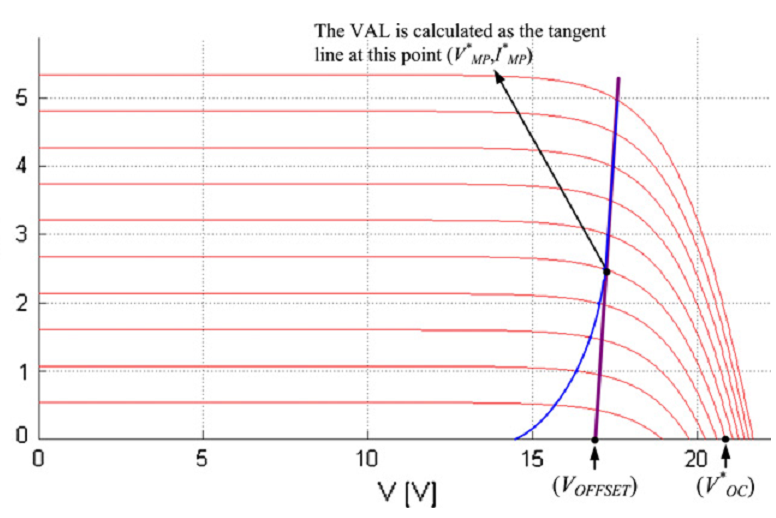
\includegraphics[width=\textwidth]{images/IVCurve_lui}
   \caption{I–V curves of the solar panel under different irradiation levels and the Voltage Approximation Line. \cite{liu2011fast} }
   \label{fig:Lui_IV_1}
   \end{center}
   \end{figure}
   
\begin{figure}[H]
    \begin{center}
         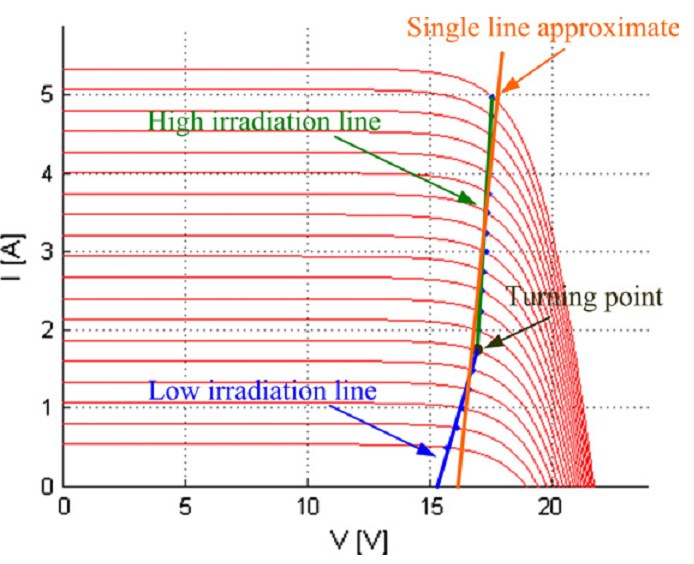
\includegraphics[height=0.4\textheight]{images/IVCurve_lui_2}
         \caption{Research Cell Efficiency Records \cite{liu2011fast} }
         \label{fig:Lui_IV_2}
    \end{center}
\end{figure}
On a cursory glance, a similar trend seems to appear on the I-V curves for the \ac{DSCs} under test (figure~\ref{fig:vmmp_lux50_5000}). Since we are restricting our study to low illuminations (indoor light conditions) we can safely discount the phenomena. This stance is also reinforced in figure \ref{fig:Probability_field} on page ~\pageref{fig:Probability_field} which shows an almost linear relationship for the light range under test but this problem may need to be revisited in case we decide to extend the algorithm for a wider window of illuminations.        
   
      
 \begin{figure}[H]
   \begin{center}
     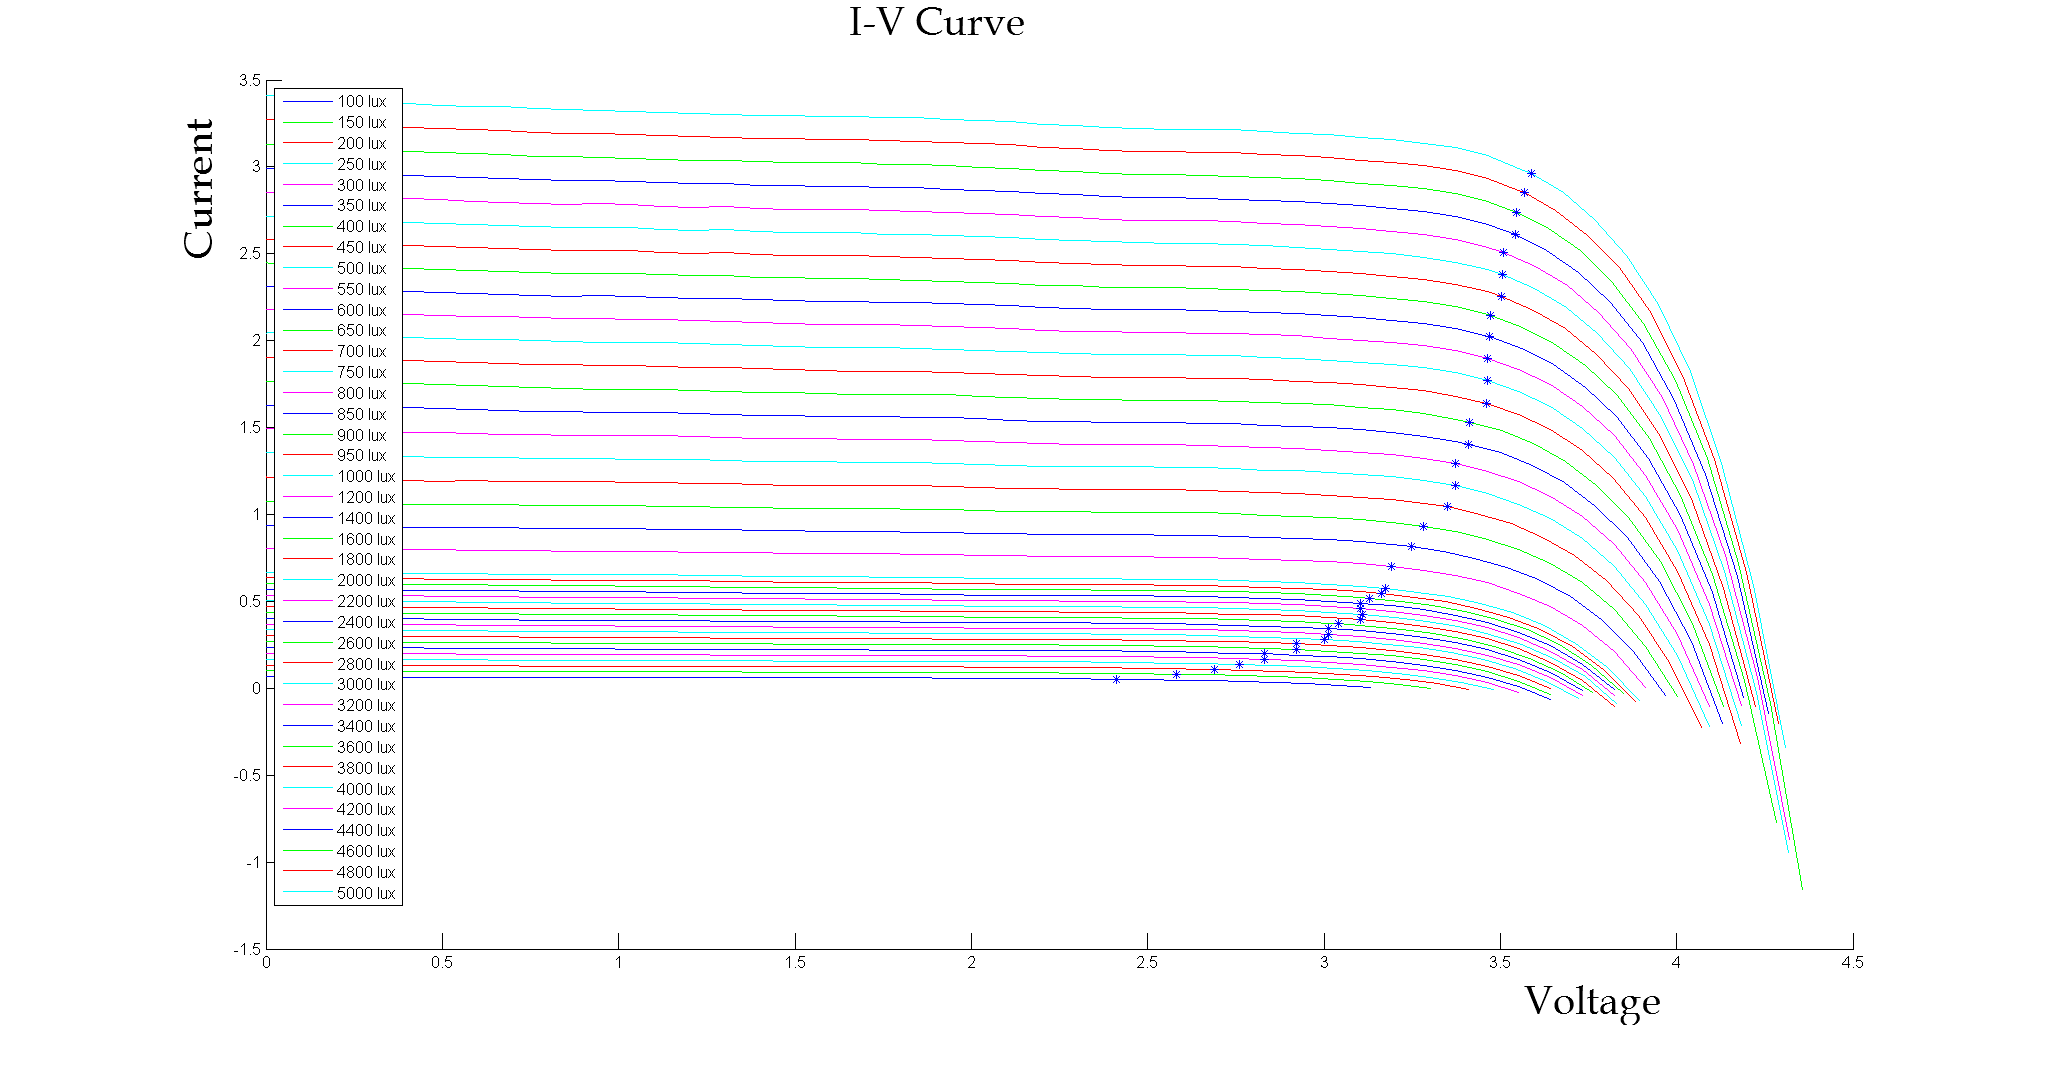
\includegraphics[width=1.2\textwidth]{images/IV_50-500}
     \caption{Variation of V\textsubscript{MPP} for different illuminations observed in the DSC under test }
     \label{fig:vmmp_lux50_5000}
   \end{center}
  \end{figure}
   
 
As discussed previously (sections \ref{sec:pno_sec} \& \ref{sec:icm_sec}), having a fixed step size has serious drawbacks; large steps lead to oscillations around \ac{MPPT} and smaller step size slows down tracking significantly, also leading to energy loss. As discussed in section~\ref{sec:others_algo}, I.Houssamo et al.~\cite{houssamo2013experimental} show the advantage of variable step tracking over fixed step based algorithms. meanwhile, S.Jain et al.~\cite{jain2004new} demonstrate a multi-stage-variable-step algorithm which involves a initial quick estimation and subsequent localization using traditional hill climbing methods (also briefly discussed in section~\ref{sec:others_algo}).\\  

 The proposed algorithm draws inspiration for the above article for its two-stage implementation to reduce the number of iterations but deviates significantly in the implementation and algorithms used to identify the \ac{MPP}.\\ 
 

Taking all prior research and findings into account; a hybrid, multi-stage, variable-step-size, self learning algorithm is proposed. The routine implements a circular buffer that acts as a look-up table, the size of the buffer can be varied as per requirement. A benefit of choosing a circular buffer is its effortless implementation of the \ac{FIFO} principle, this aids in sequentially clearing the oldest data keeping the values in the loop-up table updated and relevant. It also makes the buffer self healing, throwing out unwanted transients or errors. Since each and every solar cell is unique (even within the same batch), many having its own defects, it is highly unlikely that they exhibit the same relationship between $V\textsubscript{MPP}$ and $V\textsubscript{OC}$ as other cells. Nonetheless, $V\textsubscript{MPP}$ almost always falls between range 0.2 V and 4.0 V (the maximum $V\textsubscript{OC}$ for the illumination range). The above range forms a good starting point when the buffer is empty and the window can be made smaller with each successive successful iteration.\\

Once the outer bounds are known, \ac{GSSA} can be applied to find the maxima in relatively few steps. Every time that the \ac{MPP} is found the look-up table is updated with the new $V\textsubscript{MPP}$ and $V\textsubscript{OC}$. When the buffed does get filled up, the oldest values are discarded and replaced with the newest one.\\

Under usual operating conditions the table would always be full and equation of the line can be extrapolated using regressing modelling. For a given $V\textsubscript{OC}$ that is between the maximum and minimum open circuit voltage present in the table, the value of $V\textsubscript{MPP}$ can be easily calculated using the line equation. By taking this branch in the routine we can eliminates the use of the more costly and complex current sensor \cite{urayai2011single} by using only the voltage sensor, thereby lowering the power required to compute \ac{MPP}. This branch is also the most often taken in indoor condition where there are no drastic changes in illumination and hence $V\textsubscript{OC}$.\\  
         
In the event of a $V\textsubscript{OC}$ that is beyond the range present in the buffer, chances of its $V\textsubscript{MPP}$ lying close to the obtained line equation is very high and the same is depicted by the probability field (in blue) in figure \ref{fig:Probability_field}. The upper and lower bound of this probability field for the particular $V\textsubscript{OC}$ form the new search window for \ac{GSSA}.\\
 
Whenever branch involving \ac{GSSA} is used two sensors, current and voltage, need to be powered up in order to calculate power, so minimizing the use of this fork will increase efficiency. Cells are given a second or more to stabilize before the next iteration until \ac{MPP} is reached. If $V\textsubscript{OC}$ has remained unchanged indicating no change in incident light intensity and \ac{MPP} has been reached, then the device is put in deep-sleep conserving power only to wakeup after a specified interval to detect changes in operating parameters. Typical indoor use case imply steady, non-drastic changes in light levels, as a consequence the device is left in sleep longer. The flowchart on page ~\pageref{fig:cyflow} depicts the above routine.\\
                    
           
  \begin{figure}[H]
    \begin{center}
	   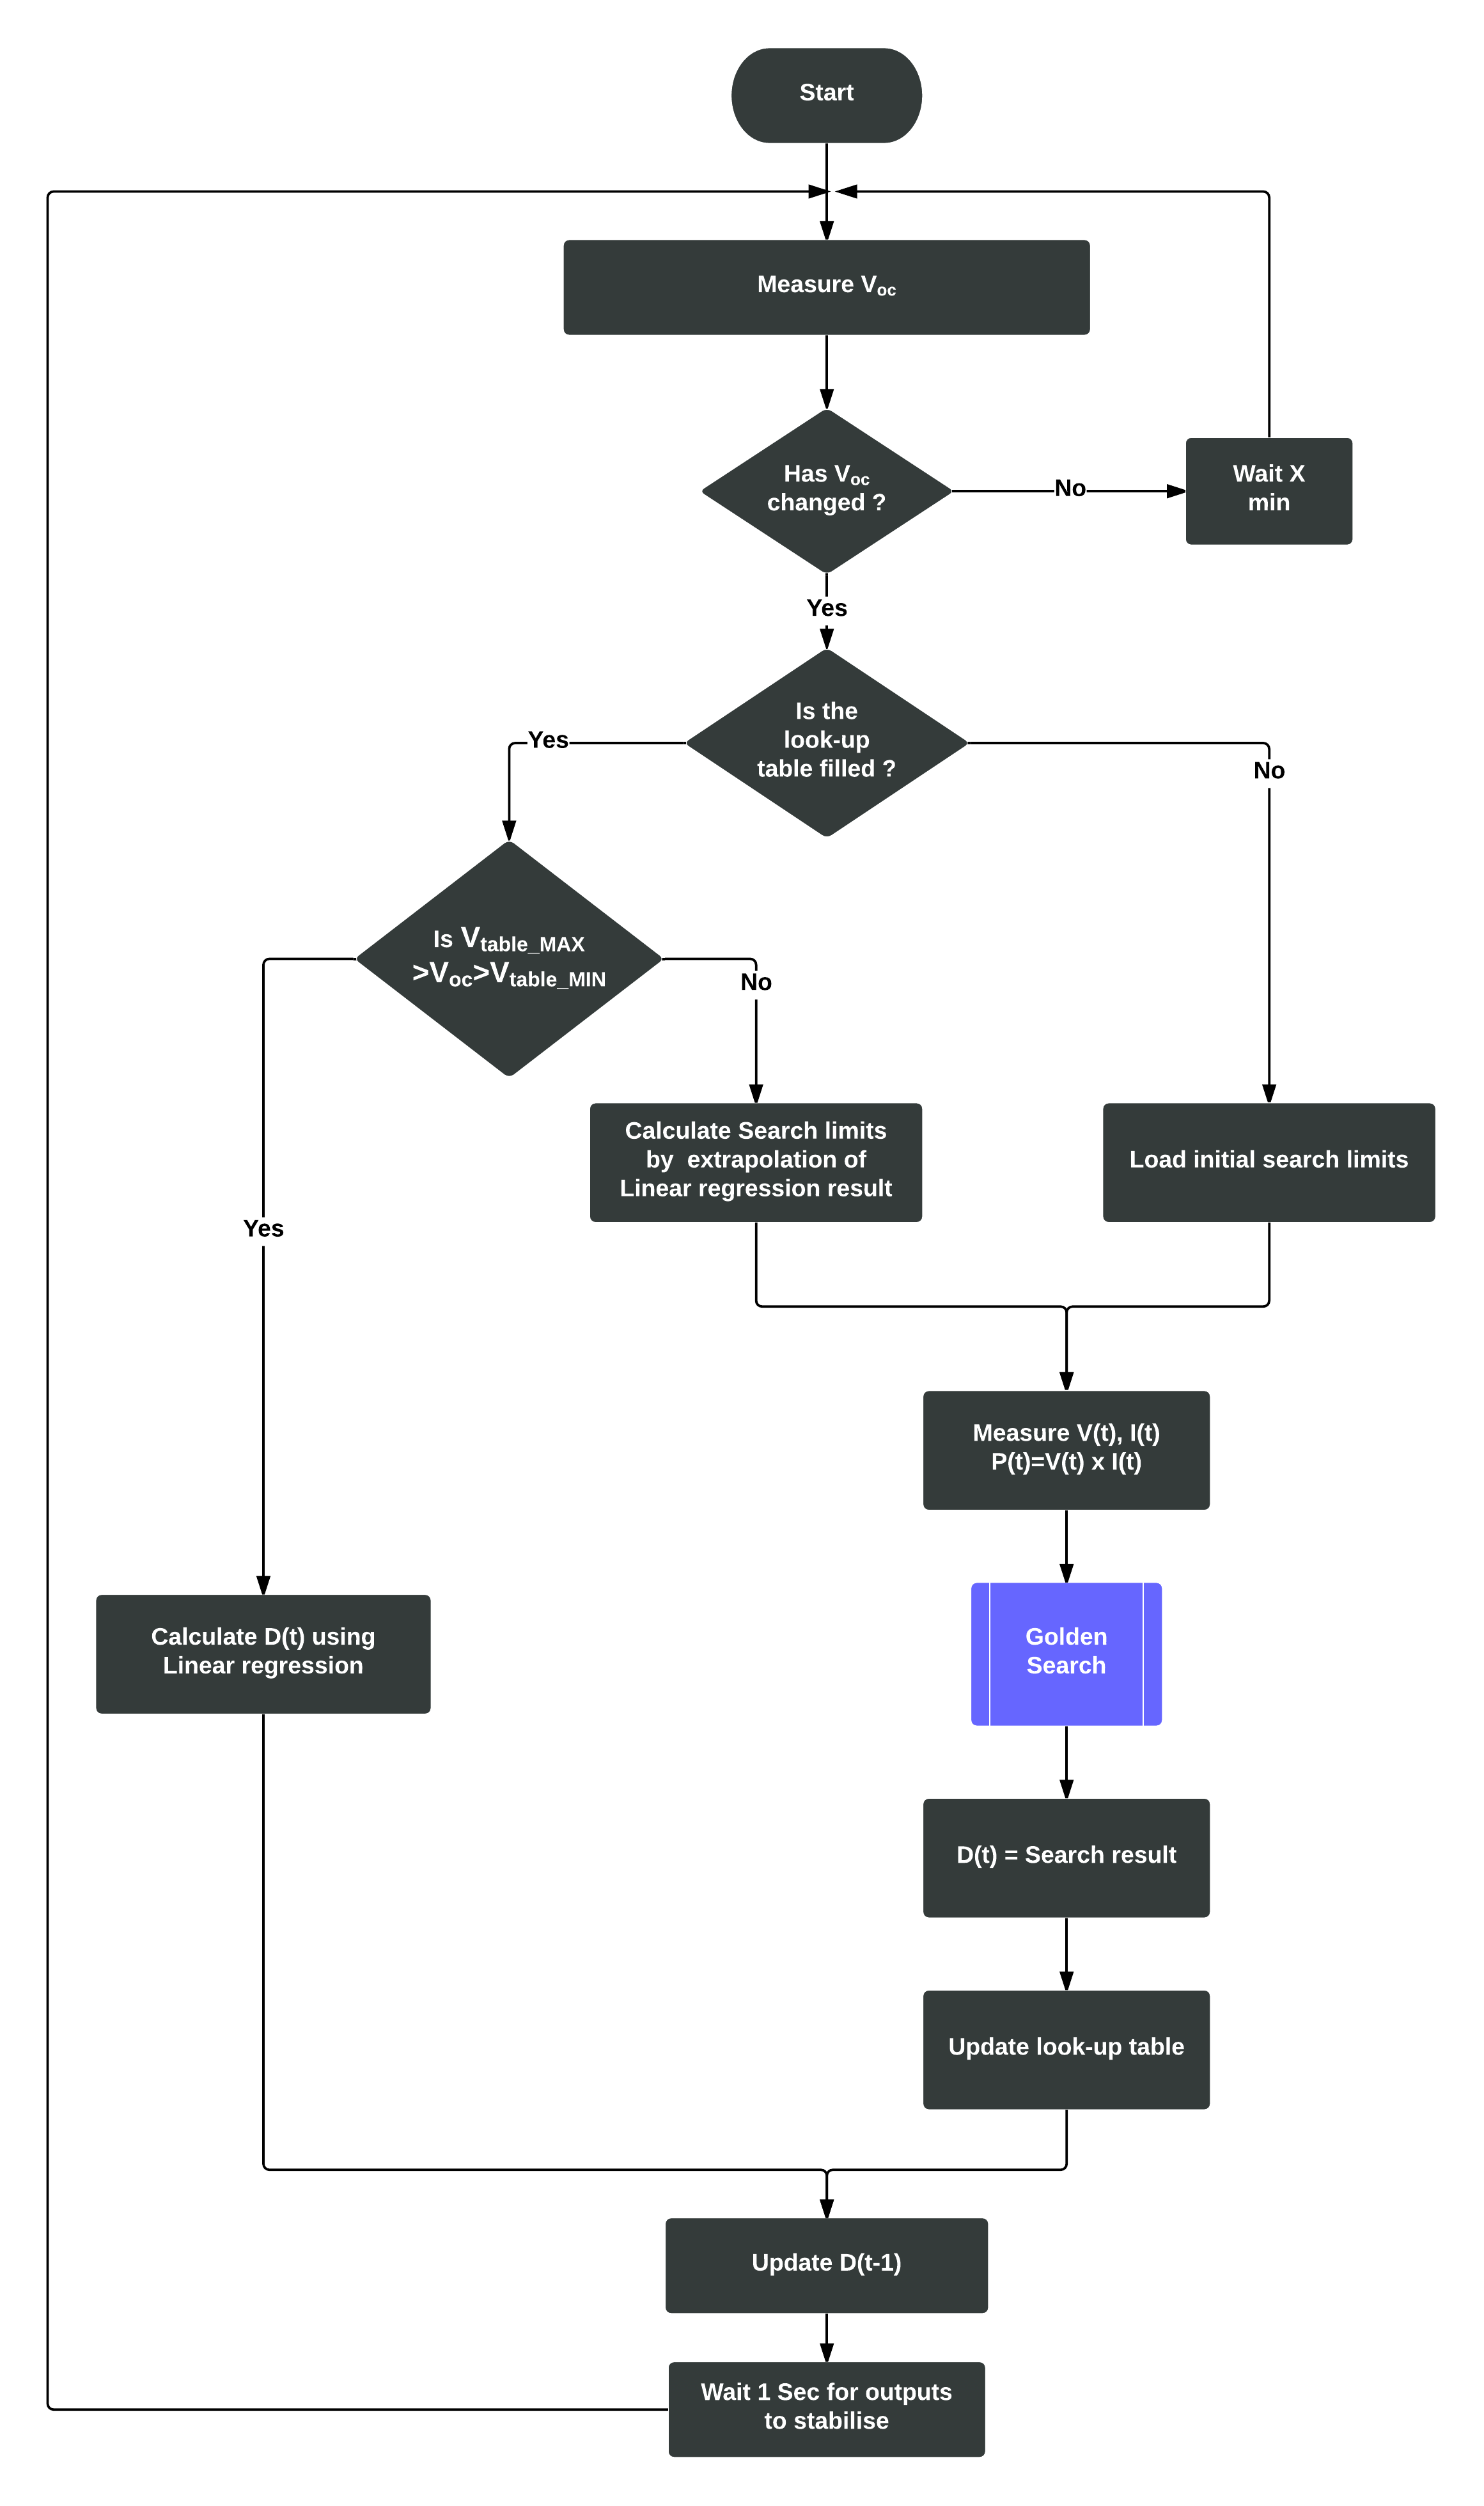
\includegraphics[width=0.9\textwidth]{images/Proposed_Flow}
	   \caption{ Flow chart for Proposed MPPT Algorithm }
	   \label{fig:cyflow}
    \end{center}
  \end{figure}





